\chapter{Motion-Aware Unitを用いた1波長を入力とした紫外線像の全球時系列予測}
  \section{実験概要}
  この実験では入力、出力ともに211Åフィルターで得られたデータを利用した。
  これは 211Åフィルターで撮影された紫外線像が、コロナホールと活動領域といった、二つの太陽円盤上の大規模構造をバランスよく明瞭に表現し、本研究のモデルの効果検証に適していると考えたためである。
  モデルにはMotion-Aware Unitを用い、1波長のデータを入力として、全球の時系列予測を行った。
  この実験の概要を図\ref{fig:exp1_overview}に示す。

  \begin{figure}[htbp]
    \centering
    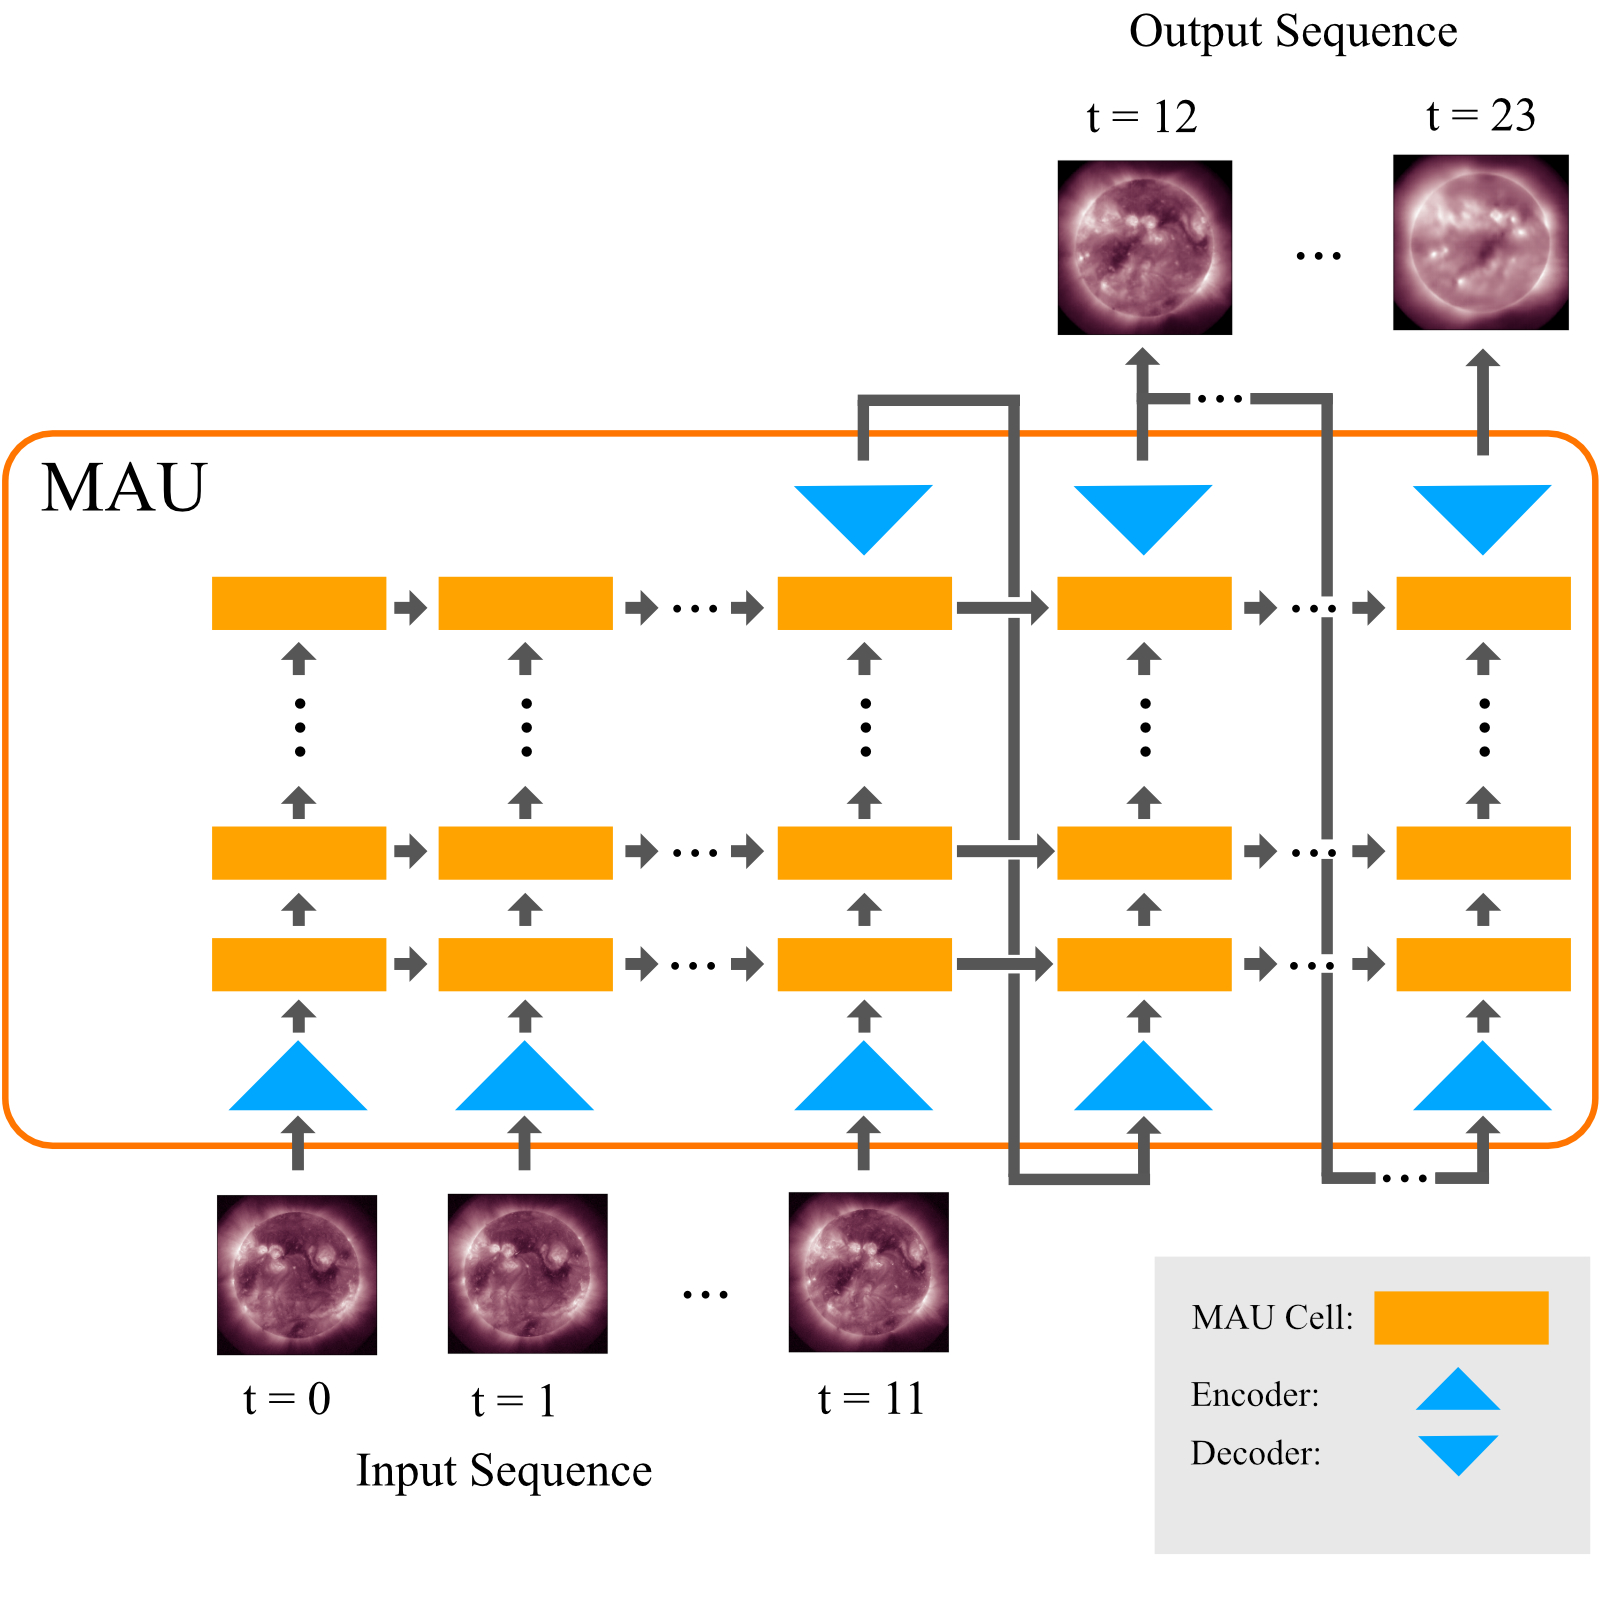
\includegraphics[width=\textwidth]{figures/exp1/exp1_concept.jpg}
    \caption{実験の概念図。モデルにはMotion-Aware Unitを用い、1波長のデータを入力として、全球の時系列予測を行った。}
    \label{fig:exp1_overview}
  \end{figure}

  \section{実験設定}
    各ハイパーパラメータの設定を表\ref{tab:exp1_hyperparameters}に示す。
    バッチサイズは実験的に決定し、最も安定的に最終的に良好な精度を達成できた値を採用した。
    また、エポック数は100とした。学習率は0.0005とした。MAU Cell数は、 \cite{chang2021mau} の実験設定を参考に、16とした。
    学習時間の短縮およびメモリ使用量の削減のため、学習時にはAutomatic Mixed Precision (AMP)(\cite{micikevicius2017mixed})を用いた。
    これは、単精度浮動小数点演算と半精度浮動小数点演算を適切に混在させることで、モデル性能をほとんど落とさずに計算資源を節約し学習を高速化する手法である。
    GPUはNVIDIA RTX A6000を用いた。
    \begin{table}[htbp]
      \centering
      \begin{tabular}{lc}
      \hline
      ハイパーパラメータ & 値 \\
      \hline\hline
      バッチサイズ & 4 \\
      \hline
      エポック数 & 100 \\
      \hline
      学習率 & 0.0005 \\
      \hline
      損失関数 & MSE \\
      \hline
      チャンネル & 1 \\
      \hline
      カーネルサイズ & (5, 5) \\
      \hline
      MAU Cell数 & 16 \\
      \hline
      \end{tabular}
      \caption{本実験でのハイパーパラメータ設定}
      \label{tab:exp1_hyperparameters}
    \end{table}

  \section{学習の推移}
  学習は図\ref{fig:exp1_learn_progress}のように推移した。
  学習損失は全体的に安定して推移し、検証損失は時折急激に値が増加しているが、全体的には減少している。
  学習の完了までには約12時間を要した。
  \begin{figure}[htbp]
    \centering
    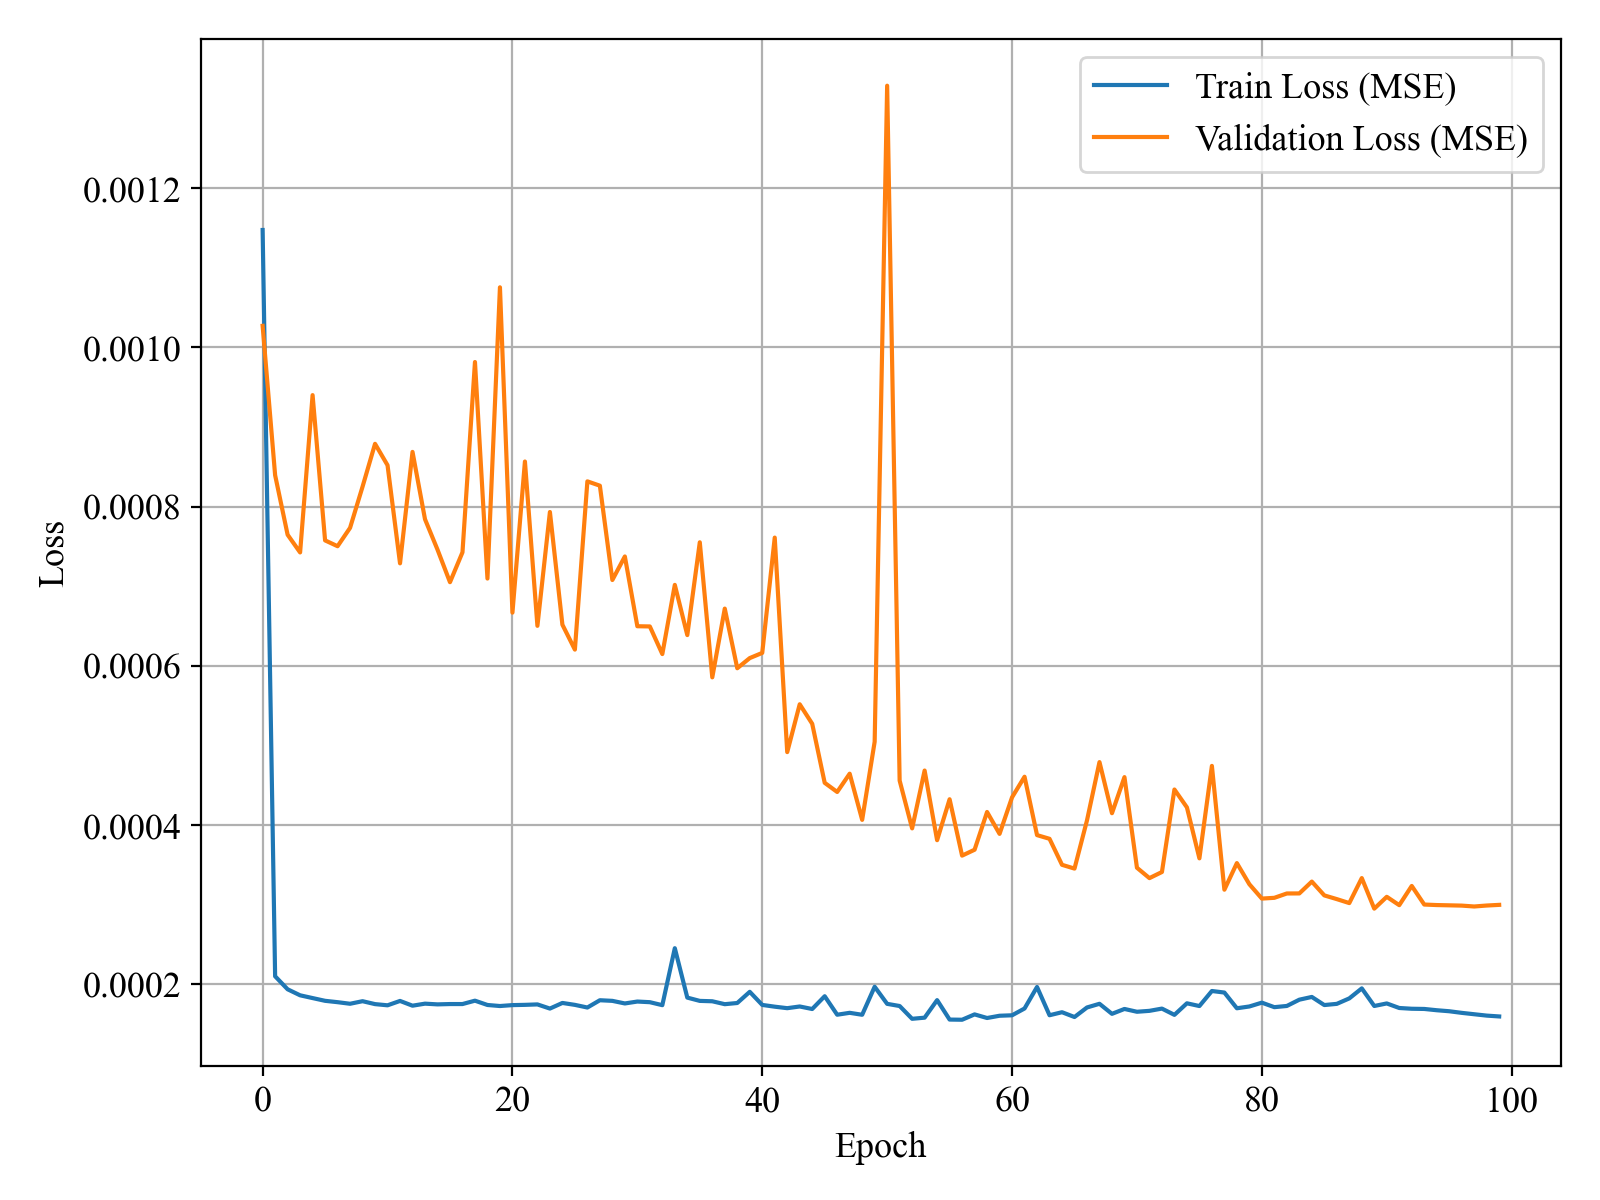
\includegraphics[width=0.8\textwidth]{figures/exp1/loss.png}
    \caption{本実験での、学習データ、検証データでの損失関数の推移。学習の損失は安定している。検証の損失は振動しながら減少している。}
    \label{fig:exp1_learn_progress}
  \end{figure}

  \section{実験結果}
    図\ref{fig:exp1_gt}および図\ref{fig:exp1_pd}に、この実験での出力例を示す。
    これは学習データに含まれない期間のテストデータである。
    \begin{figure}[htbp]
      \centering
      %\vspace*{-4cm} % 上の余白を調整
      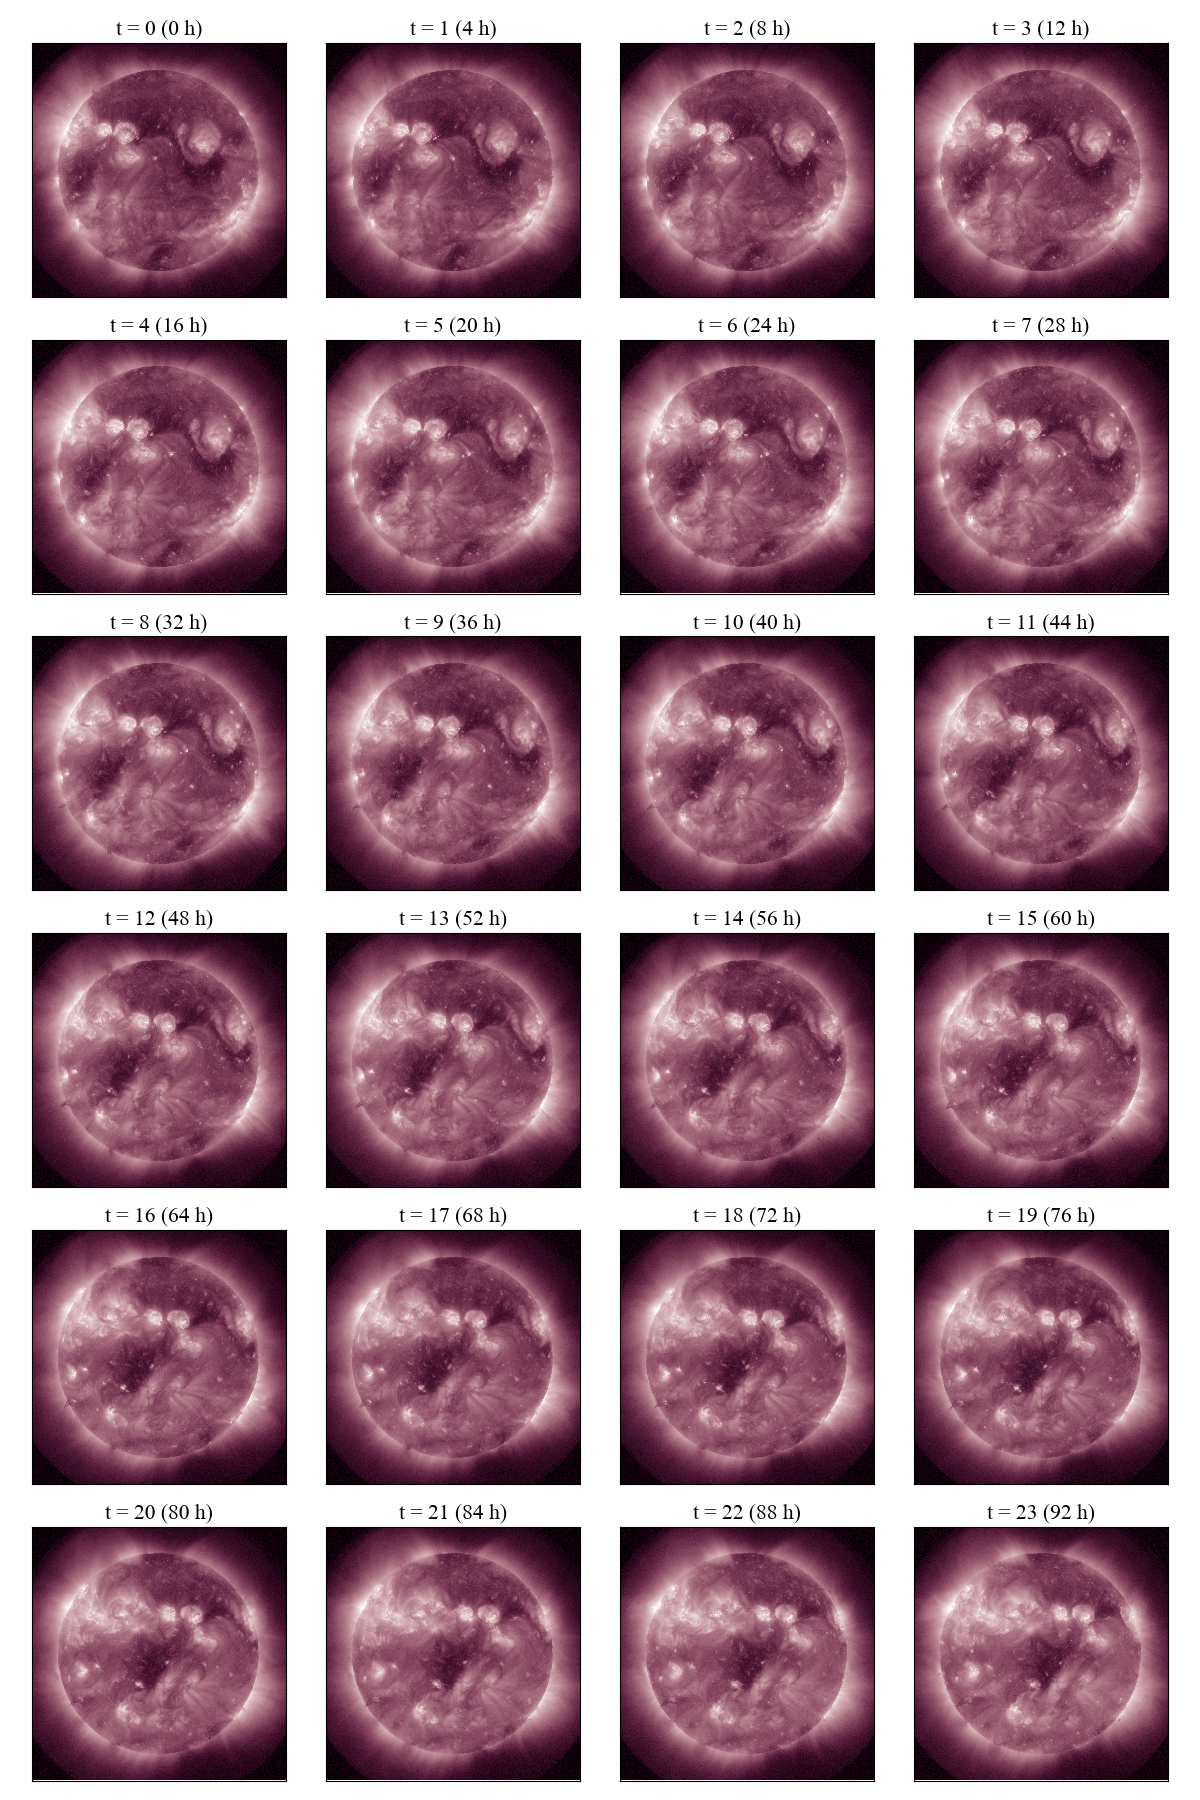
\includegraphics[width=0.95\textwidth]{figures/exp1/gt.png}
      \caption{実際の観測画像の例。2022年10月28日0時から2022年11月1日20時までの期間から4時間毎にサンプリングされている。このt=0からt=11までをモデルに入力データとして渡している。モデルはその入力データを元に、t=12からt=23の12枚の画像を予測する。t=12以降の実際の観測画像はモデルに渡されない。}
      %\vspace{-1cm} % 下の余白を調整
      \label{fig:exp1_gt}
    \end{figure}
    \begin{figure}[htbp]
      \centering
      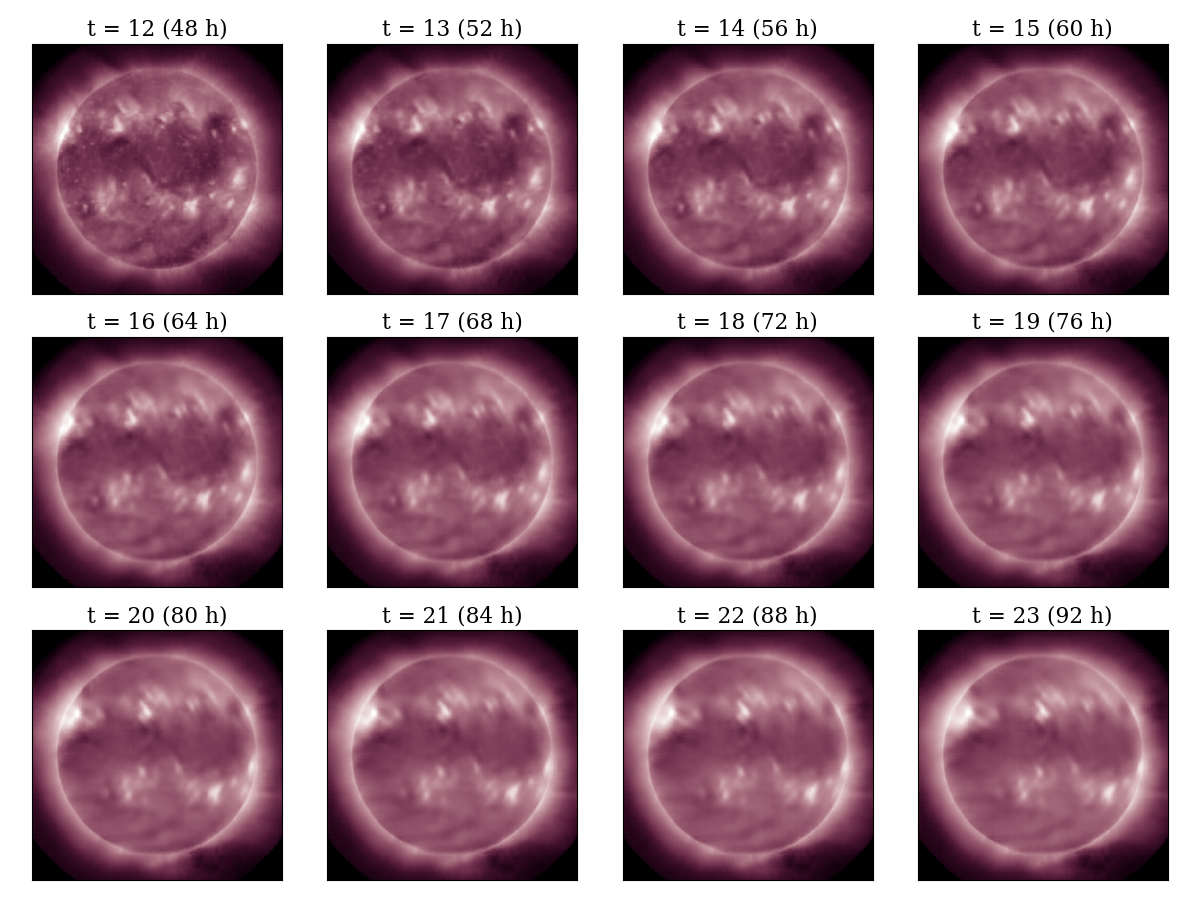
\includegraphics[width=0.95\textwidth]{figures/exp1/pd.png}
      \caption{MAUによる予測画像。対応するタイムステップtの観測画像(図\ref{fig:exp1_gt})と比較することでモデルの再現度を視覚的に評価することができる。大規模な構造は概ね実際の観測画像と合致している。モデルの特性により、時間経過とともに少しずつ予測が不安定になり、ぼやけた見た目になる。}
      \label{fig:exp1_pd}
    \end{figure}
    モデルの出力は、視覚的には実際の観測画像と概ね合致しており、特に自転による大規模構造の移動といった顕著な時間的特徴は再現できていることがわかる。

    動画予測の精度を評価するために、太陽の輝度強度の再現性を定量的、またまたは視覚的に評価する。
    これは、\citex{nishizuka2018deep} や〜〜〜などの、太陽画像から太陽イベントを予測する先行研究では、その画像中の輝度強度を主要な特徴量として採用していることに基づく。
    この輝度強度の再現性の評価を、さまざまな条件下で行った。はじめに全球での評価を行い、次に経度依存性の評価を行った。最後に、東側リムから出現する活動領域に対する視覚的評価を行った。

% *************************************************************************************************************

    \subsection{全球での評価}
      はじめに全球での評価を行った。
      この評価では、まず輝度強度の平均値と実際の平均値との誤差、構造的類似度(Structual Similarity, SSIM)を計算した。さらに単純差動回転モデルとの比較も行った。
      これらの値の時間経過に対する変化を観察し、より不確定性の高い将来の予測に対しても動画予測モデルが有効であるかを検証した。
      
      \subsubsection{平均輝度の再現}
        \paragraph{平均輝度の絶対誤差の計算}
          テストセット全体における、ある時間ステップtの平均輝度の絶対誤差を以下のように計算した。
          \begin{align}
            \bar{E}_{t} & = \frac{1}{N} \sum_{i=1}^{50} | \bar{I}_{\text{Prediction}_{i,t}} - \bar{I}_{\text{Actual}_{i,t}} |
          \end{align}
          ここで、iはテストセットのインデックスを表す。
          また、\( \bar{I}_{\text{Prediction}_{i,t}} \)は、テストセットi、時間ステップtにおける、モデルから生成された画像から計算された平均輝度を表し、\( \bar{I}_{\text{Actual}_{i,t}} \)は、実際の画像から計算された平均輝度を表す。
          平均輝度は全球(画像中の太陽の球面)に対してのみ行い、画像中の背景や外縁部からはみ出すコロナなどはその計算に含まれない。
          背景から全球に対して切り出される部分は、図\ref{fig:exp1_fulldisk_crop}に示されている。
          この全球の定義および計算は、取得したFITSファイルのヘッダーに記載される太陽の中心および半径に基づいている。
          \begin{figure}[htbp]
            \centering
            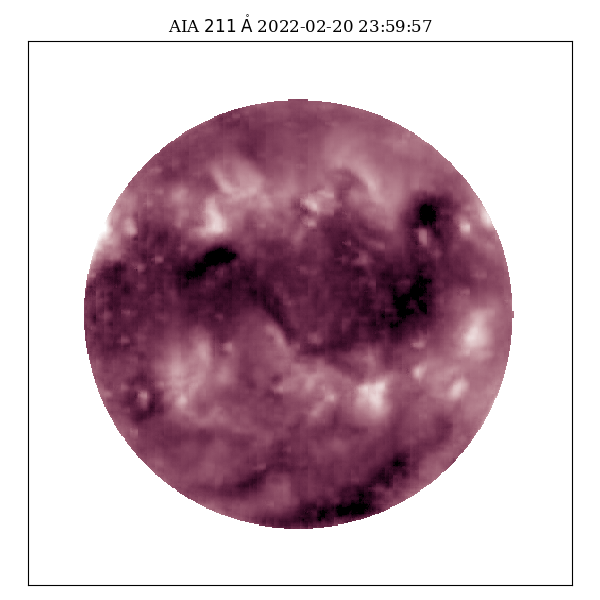
\includegraphics[width=0.6\textwidth]{figures/exp1/crop_map.png}
            \caption{生成した画像から全球部分のみ切り出した画像の例。この部分にのみ平均輝度を計算する。}
            \label{fig:exp1_fulldisk_crop}
          \end{figure}
          モデルの出力の全球での平均輝度と、実際の観測画像との誤差の推移を図\ref{fig:exp1_mean_intensity_line}に示す。
          これは、50のテストセットに対して、各テストセットに含まれる各画像の全球での平均輝度を計算し、その時間ステップごとの平均値を取ったものである。
          輝度の推移のみから特定の傾向を見出すことは難しいが、全体として平均絶対誤差は4\%以下に収まっている。
          \begin{figure}[htbp]
            \centering
            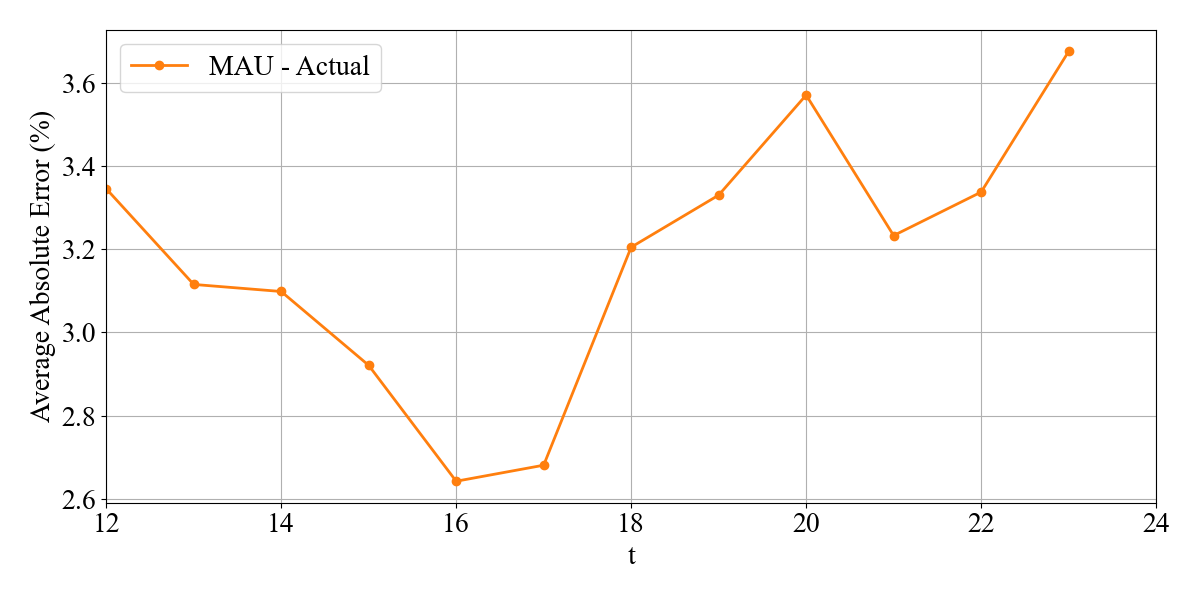
\includegraphics[width=\textwidth]{figures/exp1/error.png}
            \caption{MAUによるテストセットの予測画像と実際の観測画像の平均絶対誤差の時間推移。横軸が時間ステップ、縦軸が平均絶対誤差を表す。時間ステップを経る毎に誤差は単調に上昇していくが、その誤差は最終タイムステップでも5\%以下にとどまっている。}
            \label{fig:exp1_mean_intensity_line}
          \end{figure}
          さらに、入力シークエンスの最後から48時間後の画像の全球での平均輝度と、実際の観測画像との差異を観察する。その散布図\ref{fig:exp1_mean_intensity_scatter}に示す。
          このタイムステップは、出力の最後のタイムステップであり、最も不確定性の高い予測である。
          相関係数は0.97であり、非常に良好な値である。実際の観測画像の平均輝度の高低に関わらず、高い精度で平均輝度を再現できていることがわかる。
          \begin{figure}[htbp]
            \centering
            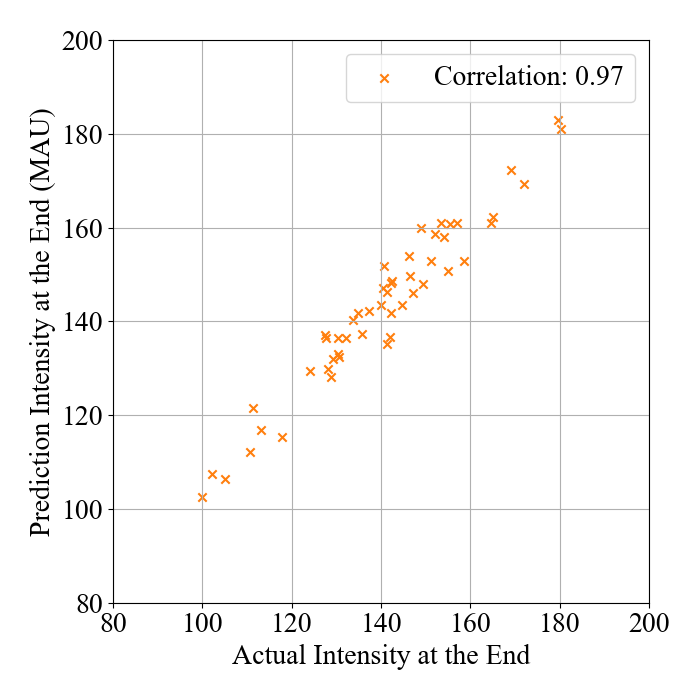
\includegraphics[width=0.6\textwidth]{figures/exp1/intensity_scatter_gt_pd.png}
            \caption{テストセットの最終ステップにおける全球平均輝度の予測対実測の散布図。縦軸がMAUによる予測から計算された平均輝度強度、横軸が実際の観測画像から計算された平均輝度強度を表す。計算された相関係数は0.97である。}
            \label{fig:exp1_mean_intensity_scatter}
          \end{figure}

        \paragraph{単純差動回転モデルとの比較}
          モデルの予測性能をさらに詳細に評価するために、シンプルな差動回転モデルとの比較を行った。
          目視や、平均輝度から、モデルの出力は実際の観測画像と概ね合致しており、特に自転による構造的変化などの主要な時間的特徴を再現できていることがわかった。
          ここでは、単純差動回転シミュレーションモデルによる出力と、我々のモデルの出力の再現精度の比較を行う。
          これにより、モデルが単に自転を予測しているのではなく、より複雑な時間的変化を予測できているかを検証した。

          太陽は自転するが、その実体は流体であるため、緯度によって自転速度が異なる。極付近の自転周期は約35日であるが、赤道付近では約25日である。この現象を差動回転と呼ぶ。
          差動回転をシミュレーションする研究は盛んに行われているが、ここでは回転速度を緯度依存としてモデル化するHoward et al. (1990) \cite{howard1990solar}の差動回転モデルを用いた。
          このモデルは、Heliographic緯度\(\theta\)に対する回転速度\(\omega(\theta)\)を以下のように定義する:
          \begin{align}
            \omega(\theta) &= A + B \sin^{2}(\theta) + C \sin^{4}(\theta) \\
            \text{where} \quad A &= 2.894 \, \mu\text{rad/s}, \\
            B &= -0.428 \, \mu\text{rad/s}, \\
            C &= -0.370 \, \mu\text{rad/s}
          \end{align}
          このモデルはSunpyに実装されており、\textit{physics.differential\_rotation}というモジュールとして提供されている。
          このモジュールによる画像の生成は、全球の各ピクセルに対して、そのピクセルの緯度に対する回転速度を計算し、その速度で西に向かって各ピクセルを移動させることで行われる。
          この単純差動回転モデルによるシミュレーションの例を図\ref{fig:exp1_sdr_example}に示す。
          このピクセルの移動による画像の生成は、全球面以外の背景には計算されない。
          また、東側外縁部からは入力にない新しい太陽表面が出現するためん、この部分は計算されない。

          比較は、単純差動回転モデルによるシミュレーションと、実際の観測画像との平均輝度の絶対誤差を計算し、それを前述の動画予測によるものと比較することで行った。
          この誤差の推移を図\ref{fig:exp1_error_sdr}に示す。単純差動回転モデルは時間経過とともに誤差が単調に増加するが、動画予測モデルは最終タイムステップにおいても誤差が4\%以下に収まっている。
          t=12から16の間は、単純差動回転モデルの方が誤差が小さいが、それ以降は逆転し、動画予測モデルの方が誤差が小さくなっている。
          このことから、動画予測モデルは、単純差動回転モデルよりも、より時間経過に対して堅牢であることがわかる。
          \begin{figure}[htbp]
            \centering
            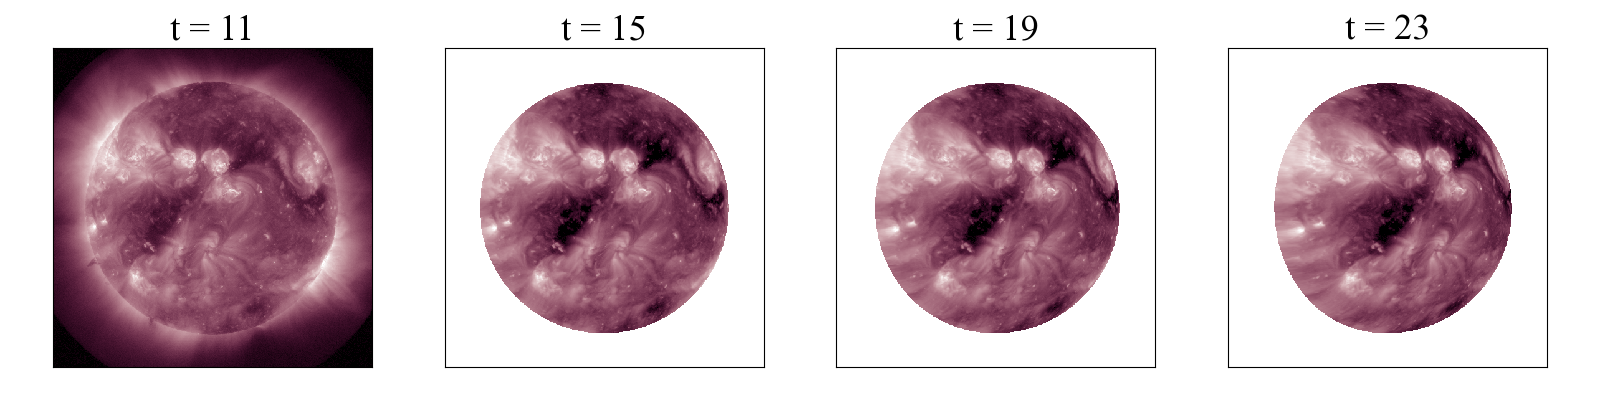
\includegraphics[width=1.1\textwidth]{figures/exp1/sdr.png}
            \caption{Howard (1990)による差動回転モデルによるシミュレーションの例。入力シークエンスの最終入力(t=11)(左)をもとに、各ピクセルに式(4.2)を適用し移動させることで画像を生成する。全球面以外の背景には計算されないため、徐々に東側から画像が欠けていくのがわかる。}
            \label{fig:exp1_sdr_example}
          \end{figure}

          \begin{figure}[htbp]
            \centering
            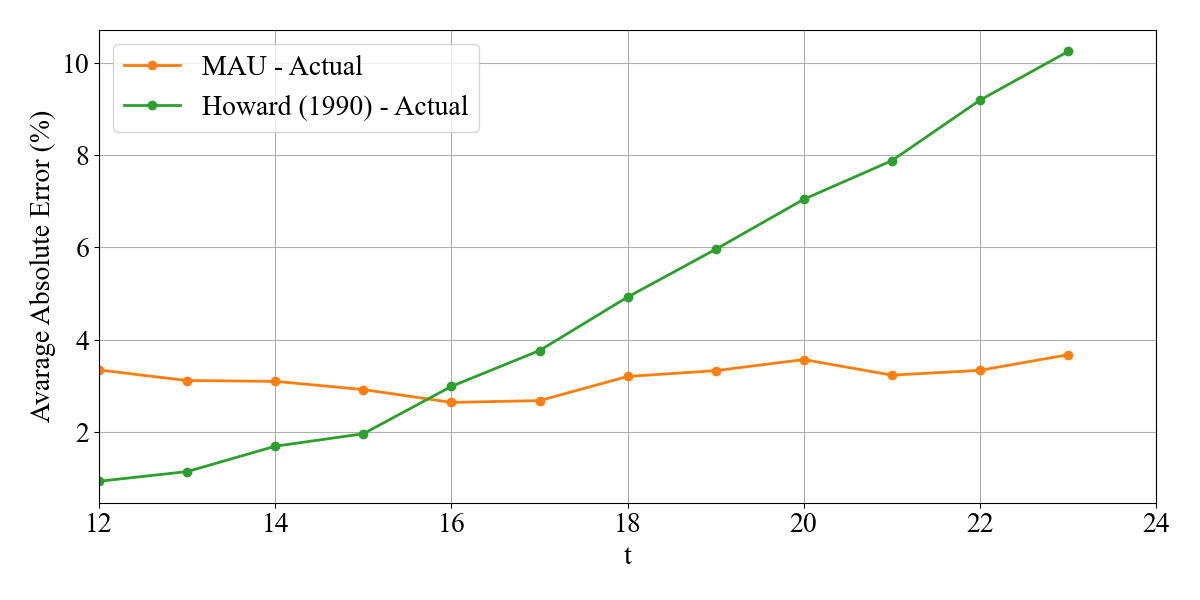
\includegraphics[width=\textwidth]{figures/exp1/error_dr.png}
            \caption{MAUによるテストセットの予測画像と実際の観測画像の平均絶対誤差(オレンジ)と、単純差動回転モデルと実際の観測画像の平均絶対誤差(緑)。}
            \label{fig:exp1_error_sdr}
          \end{figure}
          
          さらに、出力シークエンスの最後のタイムステップにおいて、単純差動回転モデルによるシミュレーションと、実際の観測画像との差異を観察し、動画予測モデルによる出力と比較した。
          その散布図\ref{fig:exp1_sdr_scatter}に示す。
          単純差動回転モデルによるシミュレーションの平均輝度と、実際の観測画像の平均輝度は、相関係数では0.85である。
          データ点が全体的に左上に偏っていることから、単純差動回転モデルは、実際の観測画像よりも平均輝度を高く予測していることがわかる。
          一方で、前述のように、動画予測モデルによる出力の平均輝度と、実際の観測画像の平均輝度は、相関係数では0.97である。
          こことから、やはり最終タイムステップでの予測においても、動画予測モデルは単純差動回転モデルよりも高い精度で平均輝度を再現できていることがわかる。
          \begin{figure}[htbp]
            \begin{subfigure}[b]{0.55\textwidth}
              \centering
              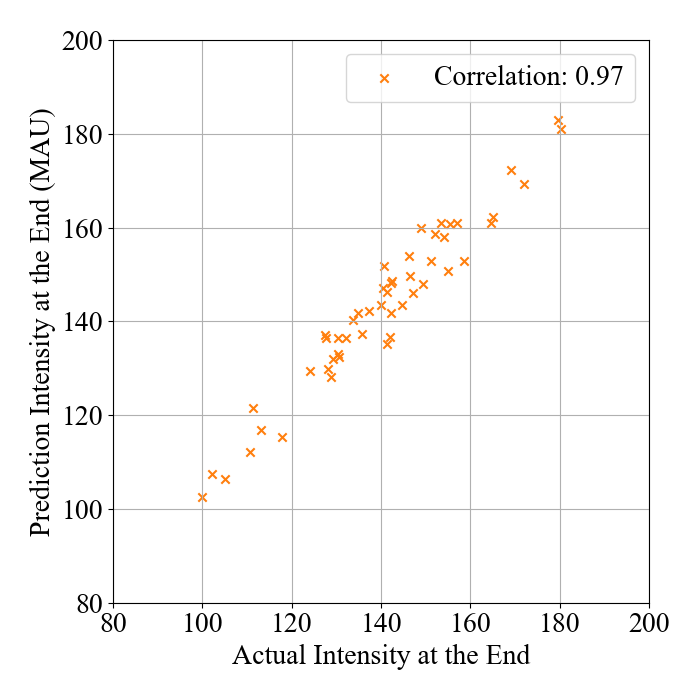
\includegraphics[width=\textwidth]{figures/exp1/intensity_scatter_gt_pd.png}
              \caption{MAUによる、テストセットの最終ステップにおける全球平均輝度の予測対実測の散布図。計算された相関係数は0.97である。}
            \end{subfigure}
            \begin{subfigure}[b]{0.55\textwidth}
              \centering
              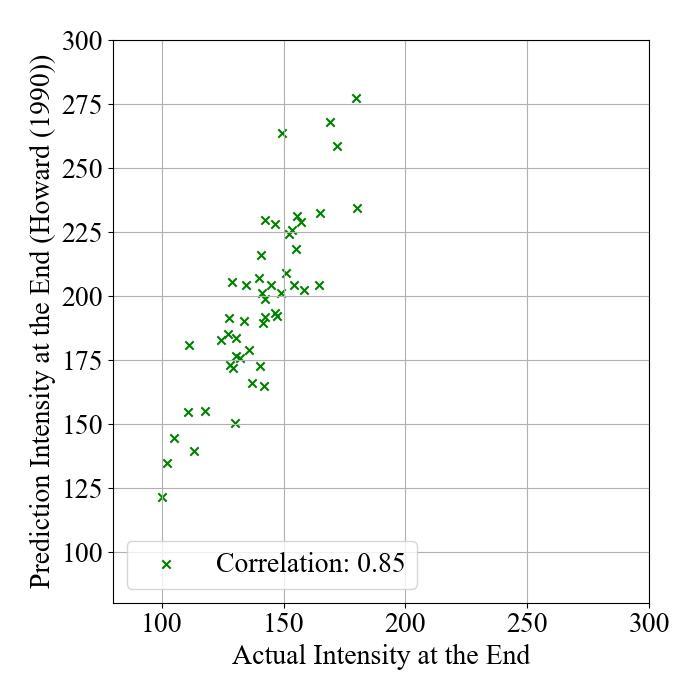
\includegraphics[width=\textwidth]{figures/exp1/intensity_scatter_gt_dr.png}
              \caption{単純差動回転モデルによる、テストセットの最終ステップにおける全球平均輝度の予測対実測の散布図。計算された相関係数は0.85である。}
            \end{subfigure}
            \caption{予測対実測の散布図。縦軸が予測から計算された平均輝度強度、横軸が実際の観測画像から計算された平均輝度強度を表す。}
            \label{fig:exp1_sdr_scatter}
          \end{figure}

      \subsubsection{画像類似度}
        画像内での構造的再現度とその時間的変化を評価するために、モデルの出力と対応する時間ステップの実際の観測画像の間のSSIMを計算した。
        SSIMは、画像の品質評価を目的として、Wang et al. (2004)\cite{wang2004image}で提案された。
        SSIMは特に構造情報が重要とされる医療画像や衛星画像のような分野で広く使用されている。従来の平均二乗誤差(MSE)やピーク信号対雑音比(PSNR)と比較して、SSIMは人間の視覚システムにより近い知覚品質を提供する。
        従来の手法とは異なり、SSIMは画像の輝度、コントラスト、構造の三つの比較を基にしている。
        SSIMの定義は以下の通りである:
        \begin{equation}
          SSIM(x, y) = \frac{(2\mu_x \mu_y + C_1)(2\sigma_{xy} + C_2)}{(\mu_x^2 + \mu_y^2 + C_1)(\sigma_x^2 + \sigma_y^2 + C_2)},     
        \end{equation}
        ここで、$x$と$y$は比較される二つの画像、$\mu_x$、$\mu_y$はそれぞれの画像の平均輝度、$\sigma_x^2$、$\sigma_y^2$はそれぞれの分散、$\sigma_{xy}$は共分散である。$C_1$と$C_2$は安定性のための小さな定数である。
        
        テストセット全体における、ある時間ステップtのSSIMの平均を以下のように計算した。
        \begin{align}
          \bar{SSIM}_{t} & = \frac{1}{N} \sum_{i=1}^{50} \text{SSIM}_{i,t}
        \end{align}

        画像類似度も、全球での平均輝度と同様に、全球に対してのみ行い、画像中の背景や外縁部からはみ出すコロナなどはその計算に含まれない。
        また、平均輝度の場合と同様に、単純差動回転モデルとの比較も同時に行った。
        このように計算されたSSIMの時間推移を図\ref{fig:exp1_ssim_line}に示す。
        MAUのSSIM、単純差動回転モデルによるSSIMは、共に時間経過とともに単調に減少していくが、MAUによるSSIMの方が、最終タイムステップにおいても0.94を超えているのに対し、単純差動回転モデルによるSSIMは0.92程度である。
        また、t=12から16の初期段階では、単純差動回転モデルの方がSSIMが高いが、それ以降は逆転し、MAUによるSSIMの方が高い。
        この傾向は平均輝度の場合と概ね同様であり、やはりMAUによる予測は画像類似度においてもその低下が緩やかである。 
        
        \begin{figure}[htbp]
          \centering
          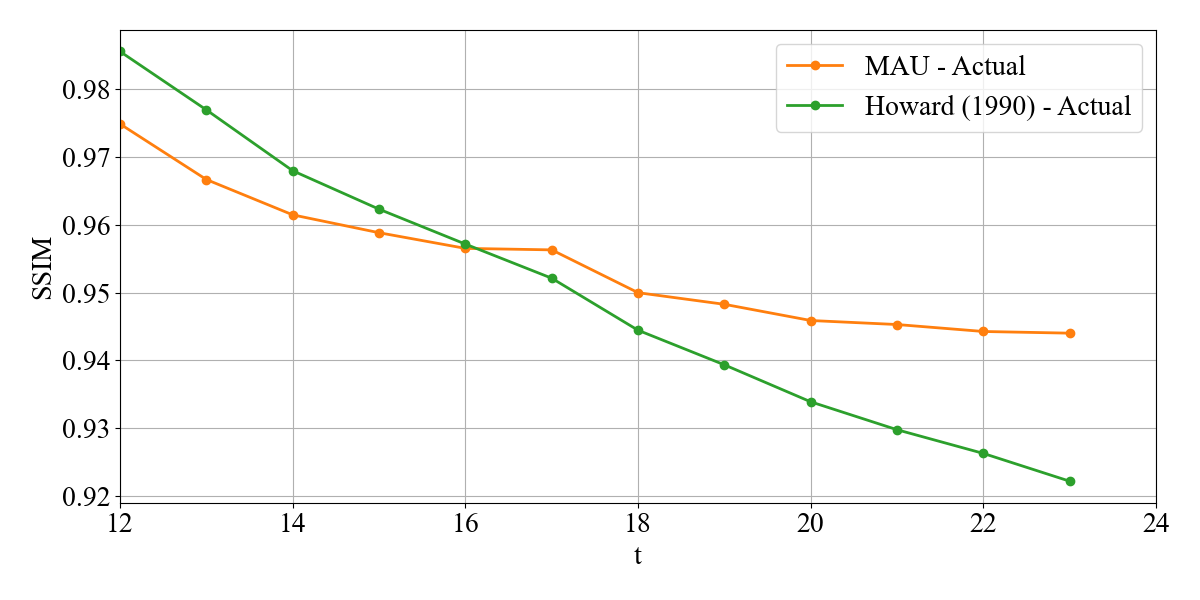
\includegraphics[width=\textwidth]{figures/exp1/average_ssim.png}
          \caption{テストセットでのSSIMの時間推移。SSIMは0から1の値を取り、二つの画像が類似するほど1に近づく。横軸が時間ステップ、縦軸がSSIMを表す。}
          \label{fig:exp1_ssim_line}
        \end{figure}
      
% *************************************************************************************************************

    \subsection{経度依存性の評価}
        さらに、予測性能が経度ごとにばらつきがあるかを確認するために、経度ごと予測の再現度を評価した。
        具体的には、Heliographic Stonyhurst座標系における経度-90°から90°までの半球を、36°ごとに5つのセクターに分割した。
        分割の概念図を図\ref{fig:exp1_division_concept}に示す。
        評価指標には、全球の場合と同様に、平均輝度の平均絶対誤差と、SSIMによる画像類似度を用いた。また、それぞれの評価において、単純差動回転モデルとの比較も行った。
        \begin{figure}[htbp]
          \centering
          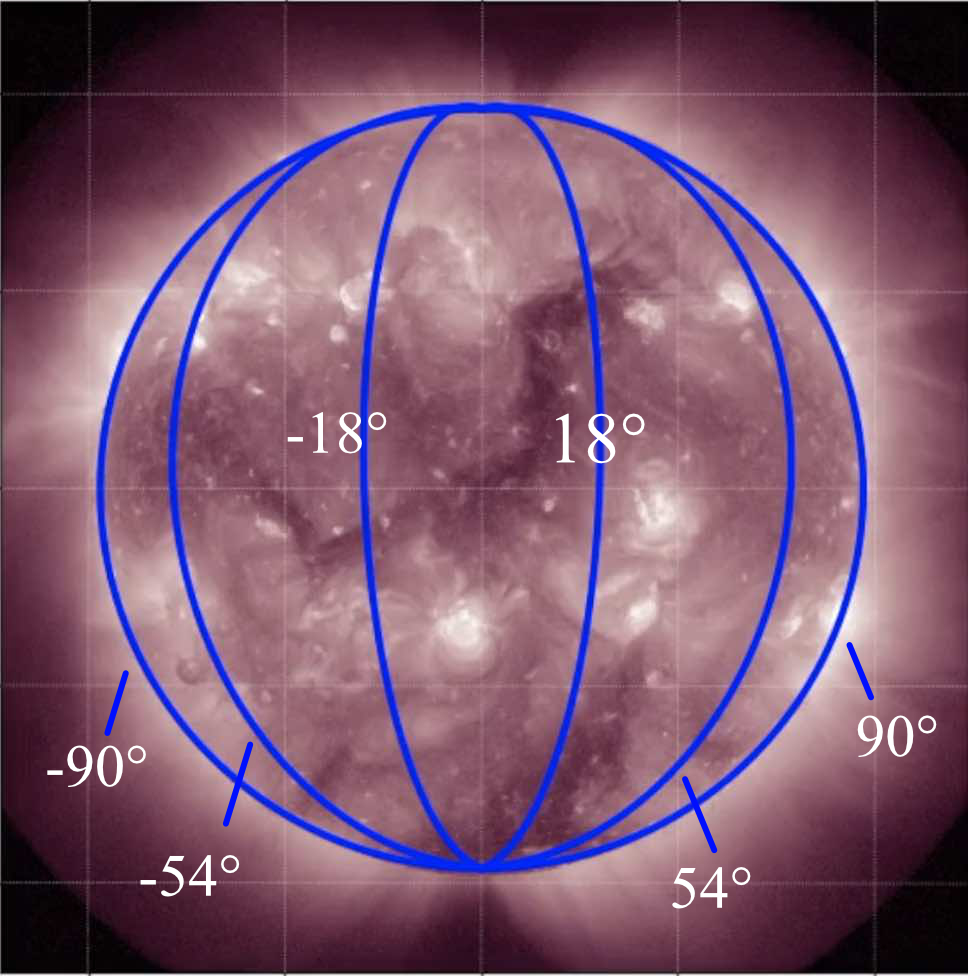
\includegraphics[width=0.65\textwidth]{figures/exp1/devision_caption.jpg}
          \caption{分割の様子を示した図。Heliographic Stonyhurst経度-90°から90°までの半球を、36°ごとに5つのセクターに分割した。}
          \label{fig:exp1_division_concept}
        \end{figure}

        \subsubsection{平均輝度の再現}
          ここでは、全てのテストセットで各セクターごとの平均輝度を計算し、対応する時間ステップの実際の観測画像との間の絶対誤差を計算した。
          ここで、ある時間ステップt、ある経度セクターlにおける平均輝度の絶対誤差\( \bar{E}_{l,t} \)は以下のように定義される:
          \begin{align}
            \bar{E}_{l, t} & = \frac{1}{N} \sum_{i=1}^{50} | \bar{I}_{\text{Prediction}_ {i, l, t}} - \bar{I}_{\text{Actual}_{i, l, t}} | \\
          \end{align}
          ここで、iはテストセットのインデックスを表す。また、\( \bar{I}_{\text{Prediction}_{i, l, t}} \)は、テストセットi、時間ステップt、経度セクターlにおける予測された平均輝度を表し、\( \bar{I}_{\text{Actual}_{i, l, t}} \)は、実際の平均輝度を表す。  
            
          このように計算された誤差率の時間推移を図\ref{fig:exp1_lng_error}に示す。
          単純差動回転モデルとの比較を行っている。
          
          \paragraph{経度-90度から-54度}
          -90度から-54度のセクターは、東の外縁部(画像に向かって左側)の領域である。
          この領域に対する誤差の推移を図\ref{fig:exp1_lng_error_1}から検証すると、MAUによる予測は、最終タイムステップで10\%程度と、全球平均の誤差率と比べると高くなっている。
          一方で、単純差動回転モデルによる予測は、最終タイムステップ80\%程度であり非常に高い。また全タイムステップにおいて、MAUによる予測よりも誤差率が高くなっている。

          しかし、単純差動回転モデルでは、新しく出現する領域に対するシミュレーションは論理的に不可能であることから、この領域に対するシミュレーション画像は時間の経過によって徐々に欠けていく。
          そのため、ここでの誤差率を比較する領域は、経度ごとの切り出しからさらに、単純差動回転モデルの出力する領域に合わせて切り取ったものとなっている。
          特に最終タイムステップt=24付近では、その領域は非常に小さくなるため、ここで計算された誤差率は、それ単体で各モデルの性能をを十分に評価できるものではない。
          そのような理由から、東側外縁部に対する評価は、ここで計算された平均輝度の絶対誤差率のみでは十分に判断できない。
          
          しかし、そのような事情を踏まえても、MAUは差動回転モデルと比較すると顕著な予測能力を示唆する誤差率を示している。
          この点については、後述する「東側外縁部に対する評価」で詳しく検証する。

          \paragraph{経度-54度から-18度}
          -54度から-18度のセクターは、東側の中心部の領域である。
          この領域は、東側外縁部と比べると、観測される面積が大きいため、より予測は容易になるものの、時間経過によって東側外縁部から移動してくる表面を予測しなければならないため、一定の難しさがある。
          ここでの誤差の推移を図\ref{fig:exp1_lng_error_2}から検証すると、MAUによる予測は、最終タイムステップで5\%程度である。
          一方で、単純差動回転モデルによる予測は、最終タイムステップで50\%程度であり、また全タイムステップにおいて、MAUによる予測よりも誤差率が高くなっている。
          このことから、東側外縁部と比べると予測が容易であるこの領域でも、予測性能の時間推移は全体的な傾向と同様であることがわかる。

          \paragraph{経度-18度から18度}
          -18度から18度のセクターは、太陽の中心部の領域である。
          この領域は、太陽の中心部であり、観測される面積が最も大きいため、予測は比較的容易であると考えられる。
          ここでの誤差の推移を図\ref{fig:exp1_lng_error_3}から検証すると、MAUによる予測も単純差動回転モデルによる予測も、全タイムステップで10\%以下であり、予測難易度は比較的高くないことがわかる。
          MAUの平均絶対誤差は、最終タイムステップで6\%であり、単純差動回転モデルが約8.5\%である。
          これから、MAUによる予測は、単純差動回転モデルよりも高い精度で予測できていることがわかる。
          
          \paragraph{経度18度から54度}
          18度から54度のセクターは、西側の中心部の領域である。
          この領域は、東側の中心部と同様に、観測される面積はある程度大きい。
          また、太陽表面が東から西に移動することから、観測できる面積の大きい太陽中心に近い領域の情報から予測を行うことができるため、東側中心部よりも予測は容易であると考えられる。
          この領域での平均絶対誤差の推移を図\ref{fig:exp1_lng_error_4}から検証する。
          MAUによる予測では、最終タイムステップで、約6\%の誤差、一方、単純差動回転モデルでは約14\%の誤差である。
          このことから、この領域においても、MAUによる予測は単純差動回転モデルよりも高い精度で予測できていることがわかる。

          \paragraph{経度54度から90度}
          54度から90度のセクターは、西側の外縁部の領域である。
          この領域は、東側の外縁部と同様に、実際の面積に対して、観測される面積が非常に小さい。
          しかし、太陽表面が東から西に移動することから、観測できる面積が大きい領域から小さい領域を予測するため、東側外縁部に比べれば予測は容易であると考えられる。
          この領域での平均絶対誤差の推移を図\ref{fig:exp1_lng_error_5}から検証する。
          MAUによる予測では、最終タイムステップで、約6\%の誤差、一方、単純差動回転モデルでは約35\%の誤差と、性能に大きな差があることがわかる。
          これは、東側外縁部と同様に、外縁部の領域においては、その予測に大きな不確実性が伴うため、単純なモデルによる決定論的な予測は困難であることを示している。
          一方で、MAUによる予測は、単純差動回転モデルよりも非常に高い精度で予測できていることがわかる。
          \begin{figure}[htbp]
            \begin{subfigure}{0.5\textwidth}
              \centering
              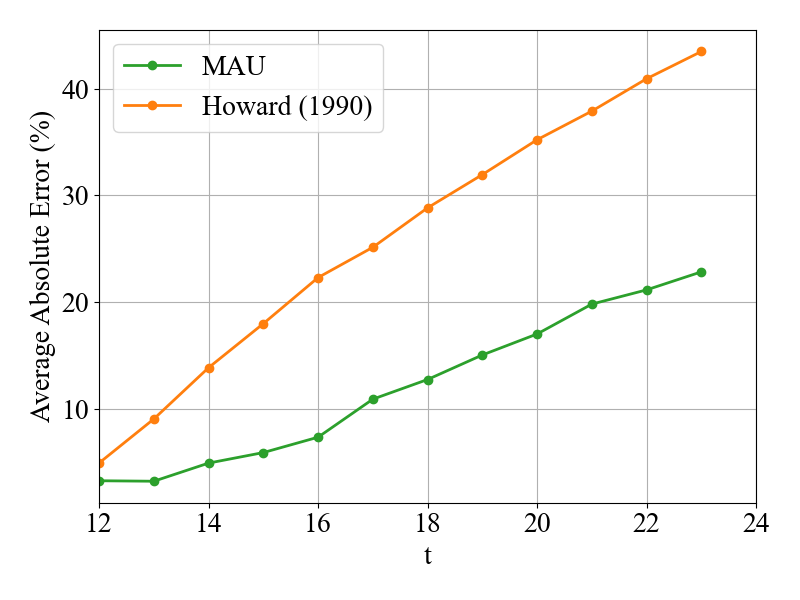
\includegraphics[width=\textwidth]{figures/exp1/lng_error_1.png}
              \caption{-90度から-54度}
              \label{fig:exp1_lng_error_1}
            \end{subfigure}
            \begin{subfigure}{0.5\textwidth}
              \centering
              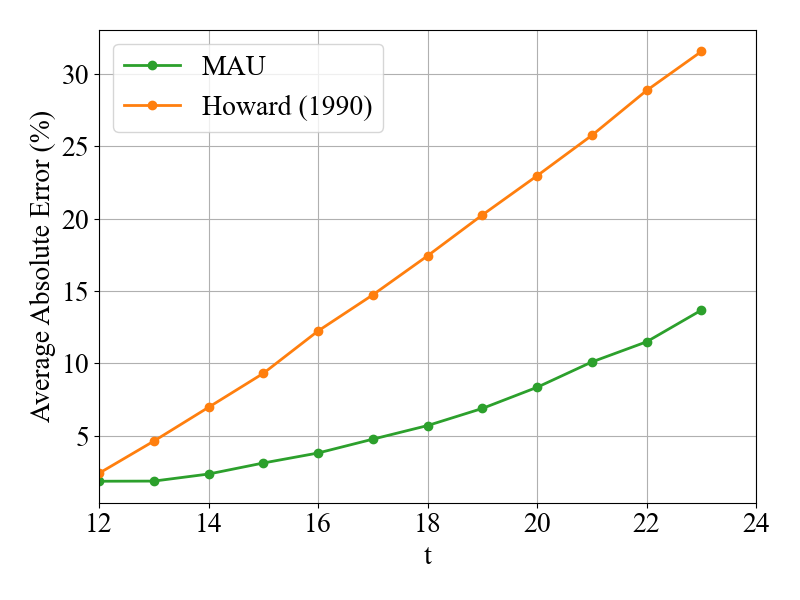
\includegraphics[width=\textwidth]{figures/exp1/lng_error_2.png}
              \caption{-54度から-18度}
              \label{fig:exp1_lng_error_2}
            \end{subfigure} \par
            \begin{subfigure}{0.5\textwidth}
              \centering
              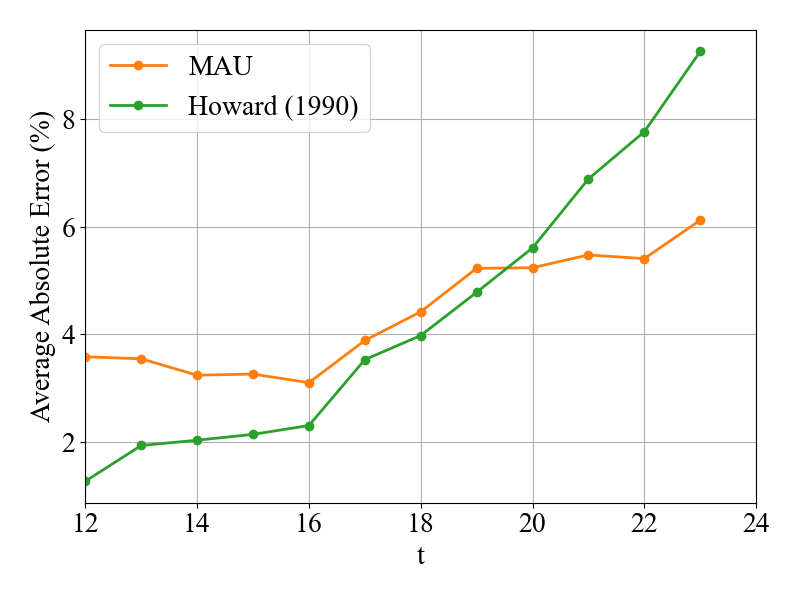
\includegraphics[width=\textwidth]{figures/exp1/lng_error_3.png}
              \caption{-18度から18度}
              \label{fig:exp1_lng_error_3}
            \end{subfigure}
            \begin{subfigure}{0.5\textwidth}
              \centering
              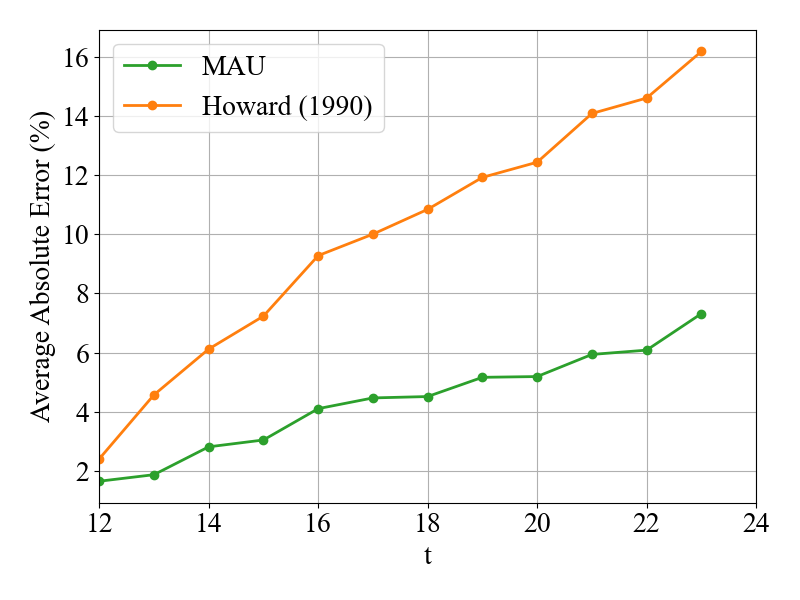
\includegraphics[width=\textwidth]{figures/exp1/lng_error_4.png}
              \caption{18度から54度}
              \label{fig:exp1_lng_error_4}
            \end{subfigure} \par
            \begin{subfigure}{0.5\textwidth}
              \centering
              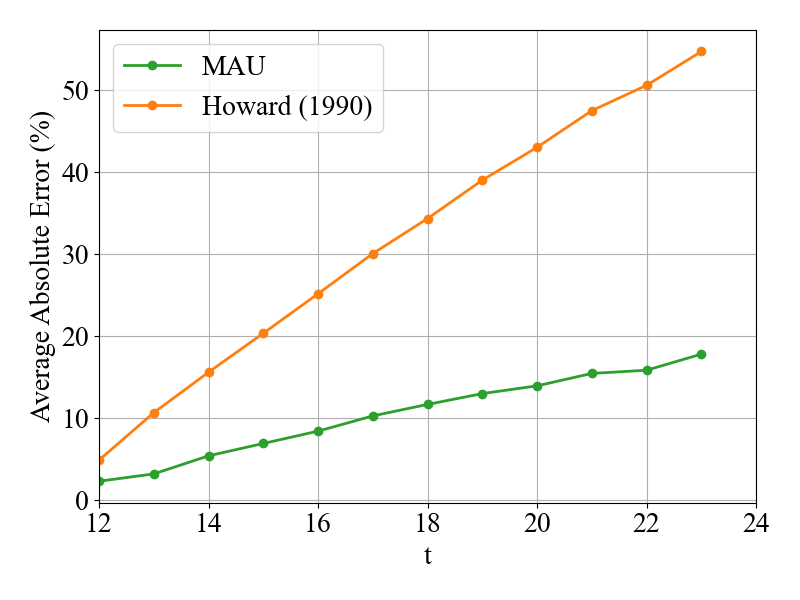
\includegraphics[width=\textwidth]{figures/exp1/lng_error_5.png}
              \caption{54度から90度}
              \label{fig:exp1_lng_error_5}
            \end{subfigure}
            \caption{分割された各セクターにおける平均輝度の絶対誤差の時間推移。横軸が時間ステップ、縦軸が平均絶対誤差を表す。各グラフで縦軸の範囲が異なる。緑線がMAUによる予測から計算された絶対誤差、オレンジ線が単純差動回転モデルによるシミュレーションから計算された絶対誤差を表す。}
            \label{fig:exp1_lng_error}
          \end{figure}
          
        \subsubsection{画像類似度}
          全球での場合と同様に、経度ごとにも画像類似度を計算した。その時間推移を図\ref{fig:exp1_lng_ssim}に示す。同時に単純差動回転モデルの経度ごとの画像類似度も計算した。
          全体的な傾向は、全球での場合と同様であり、MAUによる予測は、単純差動回転モデルよりも高い精度で予測できていることがわかる。
          特に、予測難易度の高い東側外縁部(-90度から-54度)および西側外縁部(54度から90度)において、MAUによる予測は、単純差動回転モデルの画像類似度に対して顕著な差を示している。
          \paragraph{注}
          SSIMは、実装の都合上、切り抜いた画像のみではなく、ゼロ埋めされた画像の部分も含めて計算される。
          そのため、異なる経度セクターでの比較は、画像サイズが異なるため、単純にSSIMを比較することでその経度依存の違いを評価することはできない。
          同じ経度セクターでの異なるモデルの比較は、画像サイズが同一であるため可能である。
          
          \begin{figure}[htbp]
            \begin{subfigure}{0.55\textwidth}
              \centering
              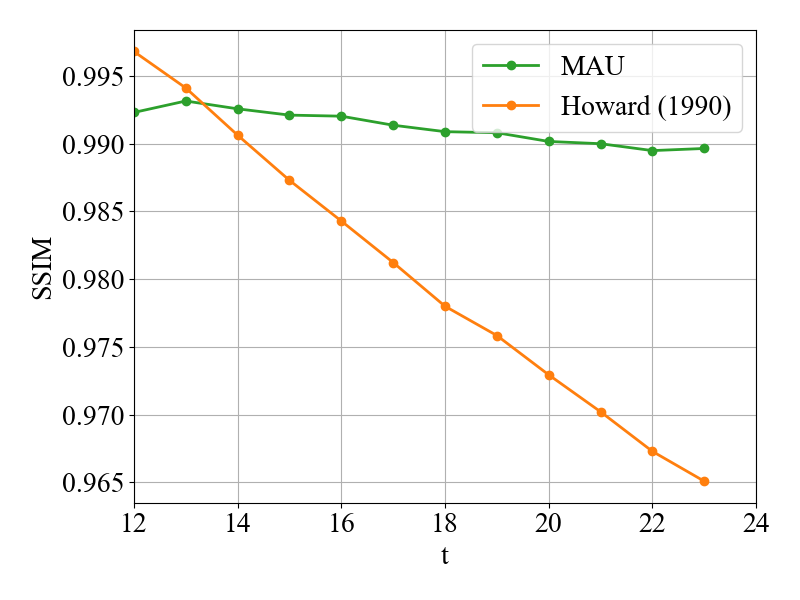
\includegraphics[width=\textwidth]{figures/exp1/lng_ssim_1.png}
              \caption{-90度から-54度}
            \end{subfigure}
            \begin{subfigure}{0.5\textwidth}
              \centering
              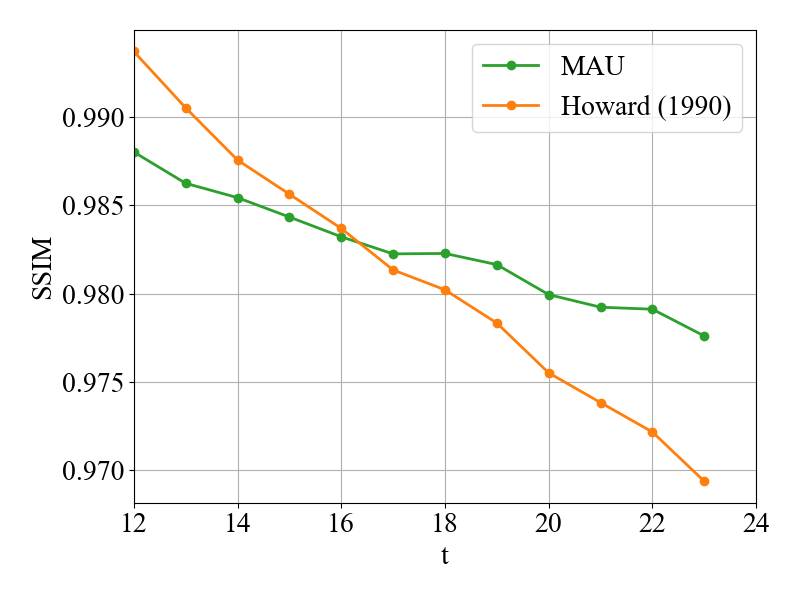
\includegraphics[width=\textwidth]{figures/exp1/lng_ssim_2.png}
              \caption{-54度から-18度}
            \end{subfigure} \par
            \begin{subfigure}{0.5\textwidth}
              \centering
              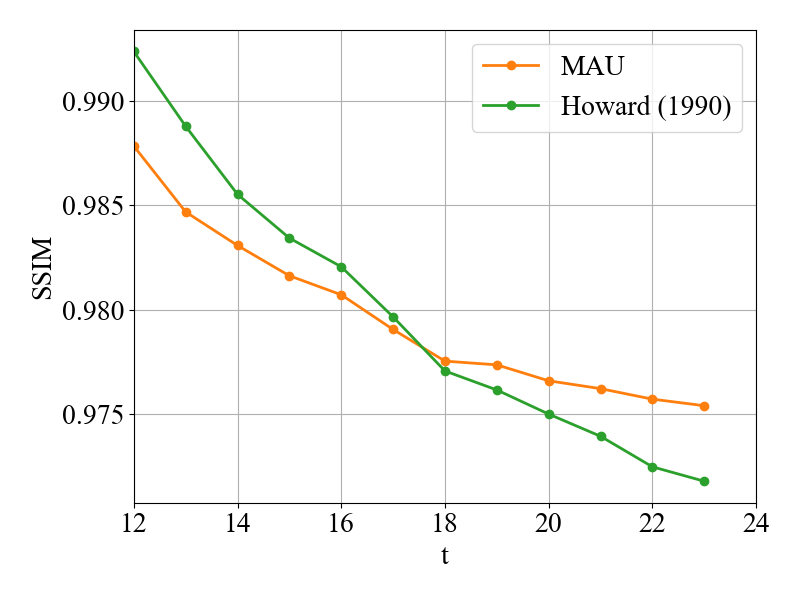
\includegraphics[width=\textwidth]{figures/exp1/lng_ssim_3.png}
              \caption{-18度から18度}
            \end{subfigure}
            \begin{subfigure}{0.5\textwidth}
              \centering
              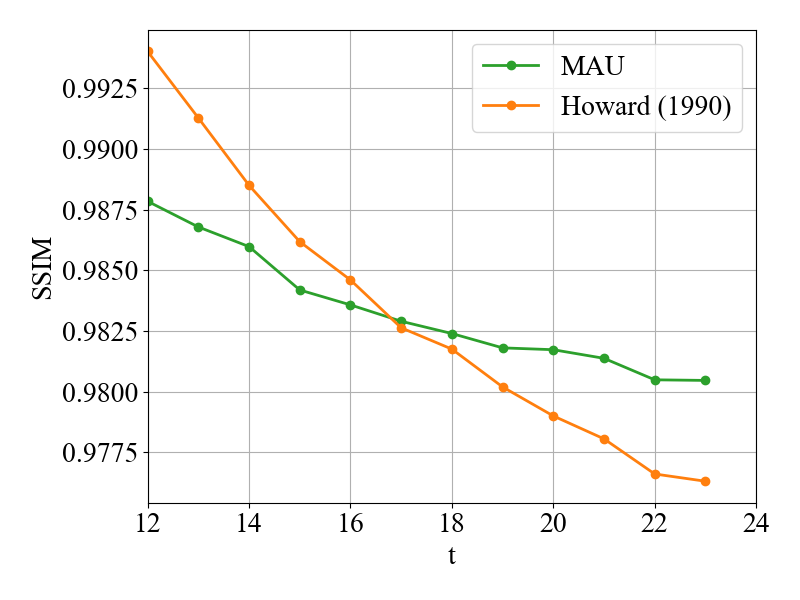
\includegraphics[width=\textwidth]{figures/exp1/lng_ssim_4.png}
              \caption{18度から54度}
            \end{subfigure} \par
            \begin{subfigure}{0.5\textwidth}
              \centering
              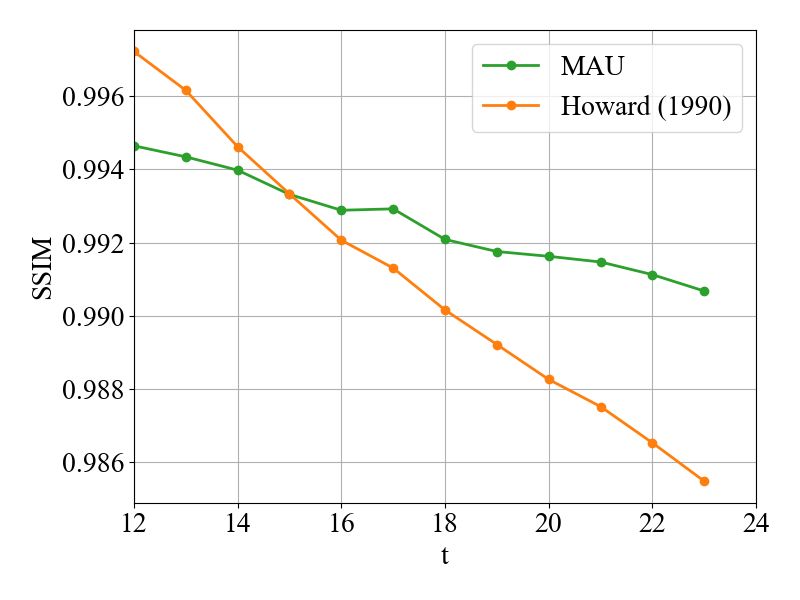
\includegraphics[width=\textwidth]{figures/exp1/lng_ssim_5.png}
              \caption{54度から90度}
            \end{subfigure}
            \caption{分割された各セクターにおけるSSIMの時間推移。横軸が時間ステップ、縦軸がSSIMを表す。各グラフで縦軸の範囲が異なる。緑線がMAUによる予測から計算されたSSIM、オレンジ線が単純差動回転モデルによるシミュレーションから計算されたSSIMを表す。}
            \label{fig:exp1_lng_ssim}
          \end{figure}

% *************************************************************************************************************
    
    \subsection{東側外縁部に対する評価}
      ここまでで、作成した動画予測モデルは、全球での平均輝度や、経度ごとの平均輝度といった定量的な評価において、実際の観測画像を正確に再現できていることを確認した。
      既存のシンプルなシミュレーションモデルとの比較でも、平均輝度の評価においては、動画予測モデルの優位性を確認できた。

      動画予測モデルのシミュレーションモデルに対するさらなる独自の特徴として、望遠鏡の視野に入っていない太陽の球面を生成することができる点が挙げられる。
      Sunpyによって提供される差動回転シミュレーションモデル\textit{physics.defferential\_rotation}は、入力された画像の全球面の各ピクセルに対して差動回転を適用することで画像を生成する。
      そのため、入力時点で望遠鏡の視野に入っていない太陽の球面を生成することができないので、より長い時間スパンでの予測を行うと、東の外縁部から徐々に予測できない領域が広がっていく。
      また、この領域は、太陽の表面が東から西に向かって回転することから、時間が経過するにつれて、望遠鏡の視野に入る領域が大きくなる領域である。
      これは、少ない情報から詳細な予測を行う必要があるため、一般的には予測が困難であると考えられる。

      これに対して、動画予測モデルは、入力画像の全球面に対して特定の数理モデルを適用するのではなく、過去のデータや全体的な文脈を元に、視野に入っていなかった領域を含む未来の状態を生成する。
      さらに、深層学習モデルは、このような不確実性の高いタスクにおいて、決定論的予測を行うシミュレーションモデルよりも有効である場合があることが知られている。
      ここでは、動画予測モデルが、そのような、入力画像の時点で全球面に見えていない領域に対して予測能力を持つか検証を行うため、生成された画像の東側外縁部から出現する活動領域に対する評価を行う。

      \subsubsection{活動領域に対する視覚的評価}
        ここでは、東側外縁部から出現する活動領域に注目して、MAUがどのような予測を行っているかを視覚的に評価する。
        予測の例を図\ref{fig:exp1_limb_example_1}および\ref{fig:exp1_limb_example_2}に示す。
        ここで示す画像は、上段が実際の観測画像、下段がその予測画像である。出現する活動領域をバウンディングボックスで囲っている。
        図\ref{fig:exp1_limb_example_1}は、活動領域が東側外縁部の北側中緯度帯から出現する例である。
        図\ref{fig:exp1_limb_example_2}は、活動領域が東側外縁部の南側中緯度帯から出現する例である。
        どちらの例においても、最終入力の時点では全球面には活動領域はほとんど出現していない。
        しかし、バウンディングボックス内を見ると、その形こそ曖昧になっているものの、活動領域の出現を予測できていることがわかる。
        \begin{figure}[htbp]
          \centering
          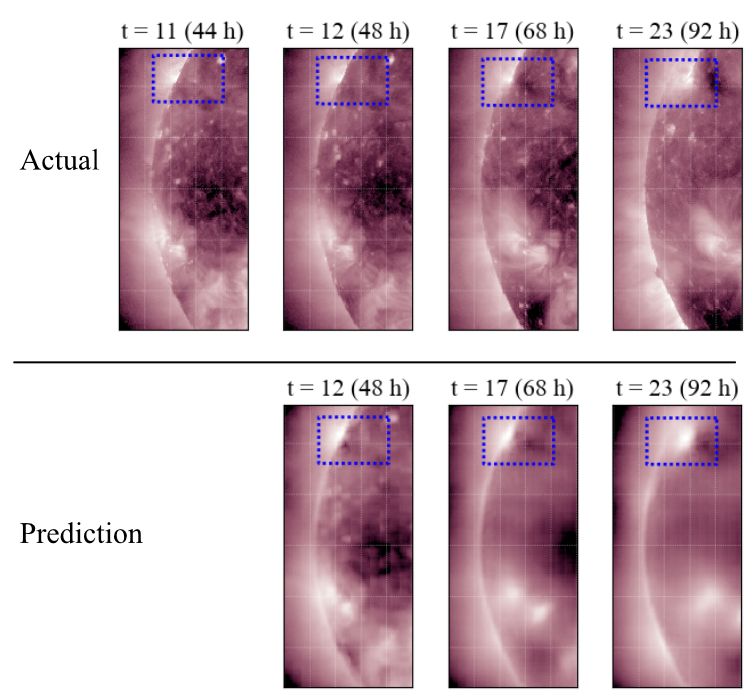
\includegraphics[width=\textwidth]{figures/exp1/limb_sample_3_caption.jpg}
          \caption{東側外縁部の北側中緯度帯から出現する活動領域をもつテストセットの例。上段が実際の観測画像、下段がその予測画像である。活動領域を青色破線のバウンディングボックスで囲んでいる。2022年11月6日0時から2022年11月9日8時の期間の画像。}
          \label{fig:exp1_limb_example_1}
        \end{figure}
        \begin{figure}[htbp]
          \centering
          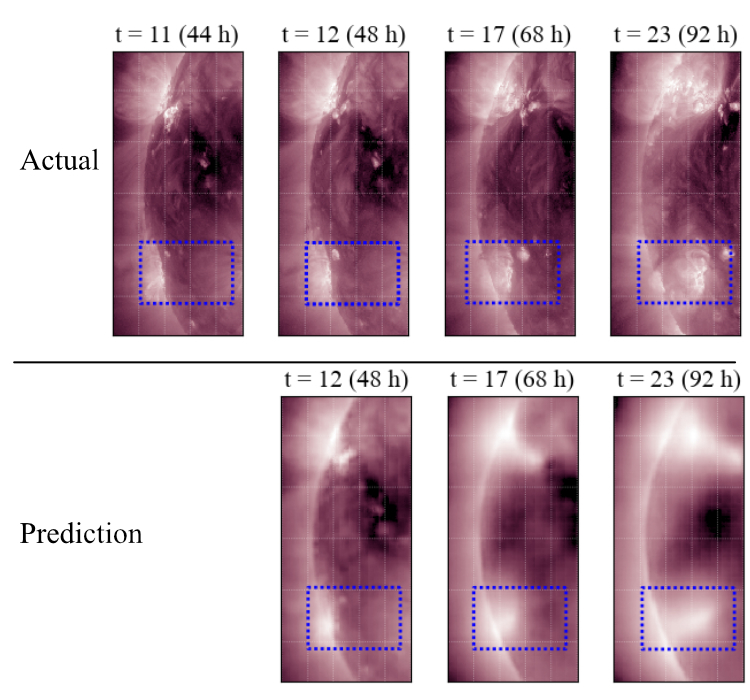
\includegraphics[width=\textwidth]{figures/exp1/limb_sample_12_caption.jpg}
          \caption{東側外縁部の南側中緯度帯から出現する活動領域をもつテストセットの例。上段が実際の観測画像、下段がその予測画像である。活動領域を青色破線のバウンディングボックスで囲んでいる。2022年12月12日0時から2022年12月15日8時の期間の画像。}
          \label{fig:exp1_limb_example_2}
        \end{figure}

      \subsubsection{予測対実測散布図による定量的評価}
        さらに、東側外縁部に対する評価を行うために、予測対実測の散布図を作成した。その結果を図\ref{fig:exp1_limb_scatter}に示す。
        左は、MAUによる予測画像の東側外縁部の平均輝度と、実際の観測画像の東側外縁部の平均輝度の散布図である。
        実際の観測画像の東側外縁部の平均輝度と、その48時間後の予測画像の東側外縁部の平均輝度は、相関係数0.98で、強い相関があることがわかる。
        また、最終タイムステップにおける実際の観測画像の東側外縁部の平均輝度強度が、その48時間の値とどのように一致しているかを示す散布図も作成した。その結果を\ref{fig:exp1_limb_scatter}右に示す。
        この散布図から、東側外縁部の平均輝度と、その48時間後の東側外縁部の平均輝度は、相関係数0.26と相関が弱く、時間経過により容易に変化することがわかる。
        これは、東側外縁部の平均輝度の変化は、単純なロジックでは予測できないことを示している。
        \begin{figure}[htbp]
          \begin{subfigure}[b]{0.53\textwidth}
            \centering
            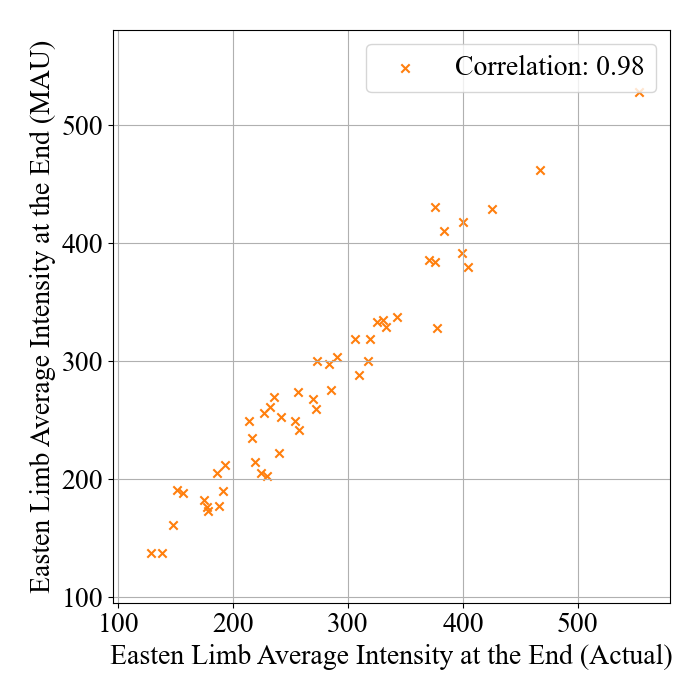
\includegraphics[width=\textwidth]{figures/exp1/limb_scatter_gt_pd.png}
            \caption{すべてのテストセットの、最終タイムステップでの東側外縁部の平均輝度の予測対実測の散布図。横軸が実際の観測画像から計算された平均輝度強度、縦軸がMAUによる予測から計算された平均輝度強度を表す。計算された相関係数は0.98である。}
          \end{subfigure}
          \begin{subfigure}[b]{0.55\textwidth}
            \centering
            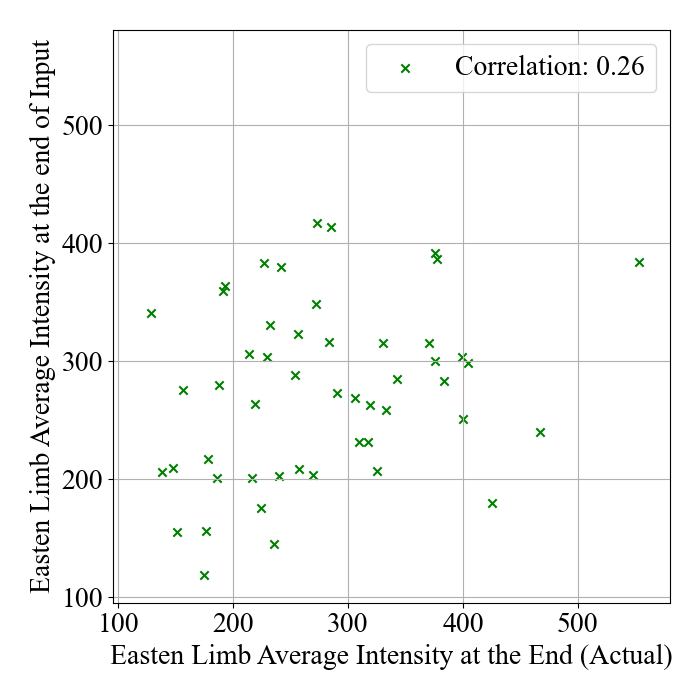
\includegraphics[width=\textwidth]{figures/exp1/limb_scatter_gt_sp.png}
            \caption{すべてのテストセットでの、最終タイムステップでの東側外縁部の平均輝度の実測値と、その48時間前の実測値の散布図。横軸が実際の観測画像から計算された平均輝度強度、縦軸がMAUによる予測から計算された平均輝度強度を表す。計算された相関係数は0.26である。}
          \end{subfigure}
          \caption{}
          \label{fig:exp1_limb_scatter}
        \end{figure}
    

  \section{考察}
    ここまでの評価結果を表\ref{tab:exp1_result}にまとめる。
    \begin{table}[htbp]
      \centering
      \caption{本実験での各評価の結果。MAUは、本研究で使用した動画予測モデルによる予測に対する評価、\citex{howard1990solar}は、単純差動回転モデルによるシミュレーションに対する評価を表す。すべての数値は、全テストセットの最終タイムステップでの値を平均したものである。}
      \begin{tabular}{lcccccc}
      \hline
      評価指標 & 全球 & \multicolumn{5}{c}{経度ごと} \\
      \cline{3-7}
       &  & -90 to -54 & -54 to -18 & -18 to 18 & 18 to 54 & 54 to 90 \\
      \hline\hline
      平均輝度絶対誤差↓ & & & & & & \\
      \quad MAU - 1波長 & 3.67 & 11.0 & 6.15 & 6.12 & 6.09 & 6.42 \\
      \quad \citex{howard1990solar} & 10.2 & 81.4 & 46.9 & 9.26 & 13.6 & 35.0 \\
      \hline
      SSIM↑ & & & & & & \\
      \quad MAU - 1波長  & 0.944 & 0.99 & 0.978 & 0.975 & 0.981 & 0.976 \\
      \quad \citex{howard1990solar} & 0.922 & 0.965 & 0.969 & 0.972 & 0.976 & 0.985 \\
      \hline
      \end{tabular}
      \label{tab:exp1_result}
    \end{table}
    さまざまな条件下でのモデルの評価結果から、動画予測モデルの有効性を確認する。
    
    \subsection{全球での性能}
      全球での評価では、平均輝度の絶対誤差とSSIMを計算し、それぞれ単純差動回転モデルのシミュレーション結果と比較を行った。
      MAUによる予測は、全タイムステップで4\%程度を下回っている。
      最終タイムステップでの予測対実測の平均輝度の相関係数は0.98であり、予測の精度は非常に高いことがわかる。
      また、単純作動回転モデルによるシミュレーション結果では、最終タイムステップでの平均輝度の絶対誤差は10\%程度である。
      
      これらの結果から、MAUは、全球の平均輝度の再現に関して有効な能力を持ち、その能力はシンプルなシミュレーションモデルよりも高いことがわかる。
      これは、モデルが太陽の差動回転に関する再現性能を持ち、太陽の表面の輝度分布の時間変化を学習できていることを示している。
    
    \subsection{経度に対するロバスト性}
      経度ごとの評価では、平均輝度の絶対誤差とSSIMを計算し、それぞれ単純差動回転モデルのシミュレーション結果と比較を行った。
      最終タイムステップでの平均輝度の絶対誤差は、MAUによる予測では、-90度から-54度で11.0\%、-54度から-18度で6.15\%、-18度から18度で6.12\%、18度から54度で6.09\%、54度から90度で6.42\%である。
      これは、単純差動回転モデルと比較すると、全球での場合よりも大きい差がついている。
      また、単純差動回転モデルは、両端の外縁部の領域では誤差が非常に大きく、中心の領域に近づくほど誤差が小さくなっている。
      しかし、MAUによる予測では、東の外縁部では11.0\%と大きくなっているもの、他の領域では6\%程度であり、大きな精度の偏りは見られない。
      このことから、MAUは、経度に対してロバストな予測能力を持つことがわかる。
      
      太陽活動は、太陽の全域にわたって多様な形で発生し、地球への影響もその活動の種類や位置によって異なるため、全経度にわたる精度の高い予測は宇宙天気予報において重要である。
      MAUが示した経度に対するロバスト性は、太陽の動的な挙動や複雑な活動パターンを理解する上での大きな利点となる。
      
    \subsection{東側外縁部における予測性能}
      東側外縁部(-90度から-54度)の最終タイムステップでの平均輝度の予測対実測の相関係数は0.98であり、高い相関を示した。
      また、視覚的評価において、東側外縁部から出現する活動領域に対して一定の予測能力を持つことがわかった。

      ベースラインとして計算した、入力シークエンスの最終タイムステップでの実際の観測データの平均輝度と、その48時間後の実際の観測データの平均輝度の相関係数は0.26であった。
      これは、東側外縁部の平均輝度は時間経過によって容易に変化することを示しており、その予測の難しさを示唆している。
      このような困難性は、以下のような要因が複合的に影響していると考えられる。
      \paragraph{新しい観測面の出現}
        太陽が西から東に自転することから、東側外縁部は常に新しい太陽表面が観測範囲に入ってくる領域である。
        予測モデルにおいては、その直前の観測データを用いて予測を行う。
        そのことから、そのデータが非常に限られており、入力データに存在しない観測面を予測しなければならない、という点は、予測の難易度を直接的に高め、その精度を低下させる可能性がある。
      \paragraph{面積の小ささと回転による増加}
        東側外縁部は、太陽の表面が望遠鏡の視野に入る角度が急になる領域である。
        そのため、実際の太陽表面の面積に対して、観測される面積が相対的に非常に小さくなる。
        その上、角度は徐々に緩やかになるため、その未来の状態を予測する場合、その少ない情報から詳細な予測を行う必要がある。
      \paragraph{角度の解釈}
        太陽の中心部では、その面が視線に対して直角に近くなるため、活動領域などの太陽表面の状態が、観測者にとって最もわかりやすい形で観測される。
        一方で、東側外縁部では、その面が視線に対して鋭角になるため、太陽表面の状態が実際の太陽表面の状態とは異なる形で観測される。
        このため、東側外縁部で得られる観測データから実際の状態を正確に推定するには、観測角度による歪みを考慮した、角度の意味的解釈が必要になる。
        これは、太陽の中央部に比べて、観測データの解析がより複雑になることを意味しており、予測モデルにとっても大きな課題となる。
      
      このような理由から、東側外縁部の予測は、その他の領域の予測よりも難しいと考えられる。
      しかし、上述のように、この領域においてもMAUは良好な予測性能を示した。
      当然他の経度分割領域と比較すると相対的には精度は劣るものの、この性能は当初の予測とは異なる結果であり、注目すべき点である。
      
      この結果について、以下のような理由が考えられる。
      \paragraph{高度な学習能力による予測の最適化}
        MAUが示した東側外縁部における予測精度は、モデルが高度な学習能力を持ち、限られた観測データからの一般化を行えることを示している。
        このような、複雑で不確実性が高く、データの少ない状況においても、未知の状態の推定が可能であることは、宇宙天気予報において重要な能力である。

      \paragraph{外縁部を越える高温プラズマからの予測}
        MAUは、図\ref{fig:limb_prediction}に示すように、全球の範囲外から外縁部を超えて観測される高温プラズマの輝きを利用して、通常は観測できない全球面の裏側に隠れた活動領域の存在を予測している可能性がある。
        太陽コロナは、太陽表面の活動状態に密接に関連しており、特に活動領域周辺では明るく輝くことが知られている。
        MAUがこの輝きと活動領域の出現のパターンを学習し、それを用いて観測されていない活動領域の位置を予測していると考えられる。
        このように、MAUは単なる表面の画像だけでなく、高温プラズマの輝きといった間接的な情報をも活用し、より正確な太陽活動の予測を行っている可能性がある。
        \begin{figure}
          \centering
          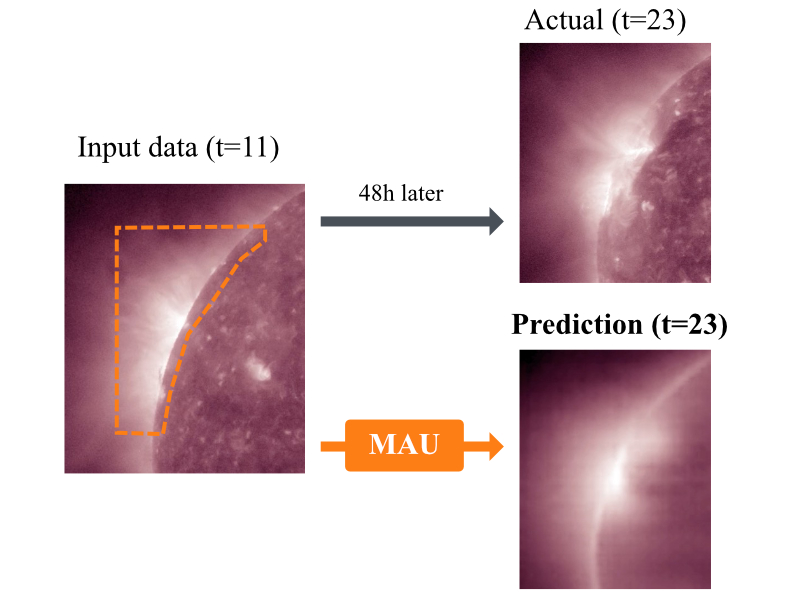
\includegraphics[width=0.85\textwidth]{figures/exp1/limb_prediction.jpg}
          \caption{}
          \label{fig:limb_prediction}
        \end{figure}

      これらの点は、MAUが差動回転などの比較的単純な現象だけではなく、太陽の物理的な特性やダイナミクスを理解し、それを基に予測を行っていることを示唆している。
    
    \subsection{複雑なシステムに対する確率的予測の有効性}
      ここでは、MAUの時間経過に対するロバスト性から、複雑なシステムを持つ太陽の表面活動に対して、確率的予測を行う深層学習モデルが有効である可能性を考察する。

      MAUによる予測画像から計算された平均輝度の絶対誤差を示した図\ref{fig:exp1_error_sdr}やSSIMを示した図\ref{fig:exp1_ssim_line}から確認すると、MAUは、時間が経過しても精度低下の傾向が単純差動回転モデルと比較して緩やかであることがわかる。
      また、出力の初期段階では単純差動回転モデルの方が誤差の小さい予測を行っている場合にも、時間経過によりMAUの予測精度が単純差動回転モデルの予測を上回っている。
      このような結果は、我々の深層学習を用いた動画予測モデルが時間経過に対してロバストな予測能力を持つことを示している。

      太陽の表面活動は非常に複雑で変動が激しいことで知られている。
      このようなシステムを物理的シミュレーションによってモデル化を行う研究は、????や????などを代表に盛んに行われている。
      これらを含む多くの物理モデルでは、特定の物理的な仮定や近似に基づいて決定論的な予測を行う。
      しかし、その複雑性やカオス的性質から、太陽全球といった広範囲にわたり完全に正確なシミュレーションを行うことは難しい。
      また、そのシミュレーションは非常に高コストであるのが一般的である。
      そのような性質により、定式化が十分に正確でない場合や、限られた計算リソースのもとに実行する場合、シミュレーションモデルは大きな誤差を含む予測を行ってしまう恐れがある。

      この状況において、MAUのような確率的予測を用いる深層学習モデルが、太陽活動の予測において新たな視点を提供する。
      MAUは、一定のぼやけを含む予測を行う。これは不確実性の表現として重要である。
      ぼやけを含むことで、視覚的なリアルさは一定程度損なわれるが、不確実性の高い領域や、長期的な時間範囲において、より最良に近い物理的数値を含む予測を行うことができる。
      これに対し、決定論的なアプローチを用いる物理的シミュレーションモデルでは、その予測にぼやけを含まないが、それは必ずしも正確な予測を行うことを意味しない。
      これは本実験の比較で用いた単純差動回転モデルが高精細ながら大きな誤差を含む予測を行っていることからも明らかである。
      動画予測モデルは、長期間にわたって視覚的にリアルで高精細な予測を行うことは難しいが、その代わりに、不確実性を考慮した予測を行うことができる。
      
      また、本研究でのMAUは、その学習の完了に10時間単位の時間と高性能なGPUを要求するが、学習済みモデルによるテストデータに対する予測は1秒未満で完了する。
      これは、スーパーコンピュータレベルの計算リソースを必要とする物理シミュレーションモデルと比較して非常に高速であり低コストである。
      この点は、迅速な予測が求められる宇宙天気予報において重要である。

      深層学習を用いた動画予測モデルのこのような特徴は、太陽活動のような複雑なシステムに対する予測として有効であり、シミュレーションモデルと比較しても一定の優位性を持つ可能性がある。
      しかし、現在の物理シミュレーションモデルは未来の状態の予測においては直接的な応用が限定的であり、太陽における物理現象の理解を深めることに主眼が置かれているという点において、動画予測モデルとは異なる目的を持つことに注意する必要がある。
      
      本実験に対するこれらの包括的な考察を通して、動画予測モデルが太陽活動の予測において有効であることを示した。
      特に、限られた情報や間接的な情報から正確でロバストな予測を行う能力は、特筆すべきものである。
      次の実験では、MAUのこのような高度な時空間データの学習能力に期待し、211Å以外の波長のデータを用いた予測を行う。
      

      %時間変化に対してもロバスト 単純差動回転と比べてもロバスト 
      %太陽はめちゃくちゃ複雑であり、系の振る舞いは不確実性を伴い、完全なシミュレーションは高コストで難しいので、確率的な予測を行う機械学習モデルが有効
      %MDHなどのより高度なシミュレーションモデルに対する優位性は比較していないので今後の課題
      %ぼやけるのは確率的予測なので仕方ない->全くぼやけないリアルな画像を追求するのは確率的予測を行う動画予測では本質的に難しい->
      % GANなどでリアルな画像を作るのはその複雑性から難しく、リアルさを追求しよとすると、実際のでデータから乖離する可能性がある->
      % 実際のデータから乖離すると、予測の精度が下がる可能性がある->予測の精度を上げるためには、リアルさを追求するのではなく、確率的予測の精度を上げることに注力するべき
